\documentclass[xcolor=dvipsnames]{beamer}\usepackage{graphicx, color}
%% maxwidth is the original width if it is less than linewidth
%% otherwise use linewidth (to make sure the graphics do not exceed the margin)
\makeatletter
\def\maxwidth{ %
  \ifdim\Gin@nat@width>\linewidth
    \linewidth
  \else
    \Gin@nat@width
  \fi
}
\makeatother

\definecolor{fgcolor}{rgb}{0.2, 0.2, 0.2}
\newcommand{\hlnumber}[1]{\textcolor[rgb]{0,0,0}{#1}}%
\newcommand{\hlfunctioncall}[1]{\textcolor[rgb]{0.501960784313725,0,0.329411764705882}{\textbf{#1}}}%
\newcommand{\hlstring}[1]{\textcolor[rgb]{0.6,0.6,1}{#1}}%
\newcommand{\hlkeyword}[1]{\textcolor[rgb]{0,0,0}{\textbf{#1}}}%
\newcommand{\hlargument}[1]{\textcolor[rgb]{0.690196078431373,0.250980392156863,0.0196078431372549}{#1}}%
\newcommand{\hlcomment}[1]{\textcolor[rgb]{0.180392156862745,0.6,0.341176470588235}{#1}}%
\newcommand{\hlroxygencomment}[1]{\textcolor[rgb]{0.43921568627451,0.47843137254902,0.701960784313725}{#1}}%
\newcommand{\hlformalargs}[1]{\textcolor[rgb]{0.690196078431373,0.250980392156863,0.0196078431372549}{#1}}%
\newcommand{\hleqformalargs}[1]{\textcolor[rgb]{0.690196078431373,0.250980392156863,0.0196078431372549}{#1}}%
\newcommand{\hlassignement}[1]{\textcolor[rgb]{0,0,0}{\textbf{#1}}}%
\newcommand{\hlpackage}[1]{\textcolor[rgb]{0.588235294117647,0.709803921568627,0.145098039215686}{#1}}%
\newcommand{\hlslot}[1]{\textit{#1}}%
\newcommand{\hlsymbol}[1]{\textcolor[rgb]{0,0,0}{#1}}%
\newcommand{\hlprompt}[1]{\textcolor[rgb]{0.2,0.2,0.2}{#1}}%

\usepackage{framed}
\makeatletter
\newenvironment{kframe}{%
 \def\at@end@of@kframe{}%
 \ifinner\ifhmode%
  \def\at@end@of@kframe{\end{minipage}}%
  \begin{minipage}{\columnwidth}%
 \fi\fi%
 \def\FrameCommand##1{\hskip\@totalleftmargin \hskip-\fboxsep
 \colorbox{shadecolor}{##1}\hskip-\fboxsep
     % There is no \\@totalrightmargin, so:
     \hskip-\linewidth \hskip-\@totalleftmargin \hskip\columnwidth}%
 \MakeFramed {\advance\hsize-\width
   \@totalleftmargin\z@ \linewidth\hsize
   \@setminipage}}%
 {\par\unskip\endMakeFramed%
 \at@end@of@kframe}
\makeatother

\definecolor{shadecolor}{rgb}{.97, .97, .97}
\definecolor{messagecolor}{rgb}{0, 0, 0}
\definecolor{warningcolor}{rgb}{1, 0, 1}
\definecolor{errorcolor}{rgb}{1, 0, 0}
\newenvironment{knitrout}{}{} % an empty environment to be redefined in TeX

\usepackage{alltt}
%%\usepackage[dvipsnames]{xcolor}

\usefonttheme[onlymath]{serif}

\setbeamercolor{title}{fg=black}
\setbeamercolor{frametitle}{fg=black}

\setbeamertemplate{itemize items}[circle] 
\setbeamercolor{itemize item}{fg=black}
\IfFileExists{upquote.sty}{\usepackage{upquote}}{} 
\begin{document}

\title{R, Reserving, Linear Regression \& MRMR}
\author{Brian A. Fannin}

\maketitle

% very important to use option [fragile] for frames containing code output!




\begin{frame} {Agenda}
  \begin{itemize}
    \item Introducing MRMR
    \item Data visualization 
    \item Linear modeling
    \item Fit diagnostics
    \item Projection
    \item Another view of regression
    \item Further
  \end{itemize}
\end{frame}

\begin{frame} {Introducing MRMR}
  MRMR is another R package for use in analyzing reserves.
  
  MRMR was heavily influenced by the following:
  \begin{itemize}
    \item Andrew Gelman and Jennifer Hill, "Data Analysis Using Regression and Multilevel/Hierarchical Models"
    \item ggplot2 and Hadley Wickham
    \item Leigh Halliwell and Judge et al
  \end{itemize}
\end{frame}

\begin{frame} {MRMR Structure}
  MRMR supports three S4 classes: Triangle, TriangleModel and TriangleProjection. These have a rough correspondence to the behavior of functions lm, glm and lme4.
  
  \begin{tabular} { | l | l | l | }
    \hline
     & R & MRMR \\ \hline
    Data storage & Data frame & Triangle \\ \hline
    Model & Function lm (S3 object) & TriangleModel \\ \hline
    Project & Function predict (vector) & TriangleProjection \\ 
    \hline
  \end{tabular}
\end{frame}

\begin{frame}[fragile]{Startup MRMR}
\begin{knitrout}
\definecolor{shadecolor}{rgb}{0.969, 0.969, 0.969}\color{fgcolor}\begin{kframe}
\begin{alltt}
\hlfunctioncall{library}(MRMR)
`?`(MRMR)
\end{alltt}
\end{kframe}
\end{knitrout}




\end{frame}

\begin{frame}{Basic requirements}
  A triangle object must possess the following data elements:
  \begin{itemize}
    \item Temporal dimensions for origin period, development lag and evaluation date. These are stored as lubridate objects.
    \item Measures
      \begin{itemize}
        \item Stochastic - Loss, claim, etc. These are time series variables and candidates for prediction. MRMR will adjust these so that incremental, cumulative and prior cumulative columns are formed.
        \item Static - Typically exposure variables. These will not be adjusted. These are very good candidates for predictors.
      \end{itemize}
    \item One or more grouping elements. This is currently not implemented, but is reserved for future use.
  \end{itemize}
\end{frame}

\begin{frame}[fragile]{A brief word about lubridate}
lubridate is a package with many routines to aid in working with dates. 
\end{frame}

\begin{frame}[fragile]{lubridate examples}
\begin{knitrout}
\definecolor{shadecolor}{rgb}{0.969, 0.969, 0.969}\color{fgcolor}\begin{kframe}
\begin{alltt}
aDate = \hlfunctioncall{mdy}(\hlstring{"06-30-2012"})
\hlfunctioncall{day}(aDate) = 6
aDate + \hlfunctioncall{years}(1)
\end{alltt}
\begin{verbatim}
## [1] "2013-06-06 UTC"
\end{verbatim}
\begin{alltt}
myPeriod = \hlfunctioncall{months}(6)
myPeriod/\hlfunctioncall{months}(1)
\end{alltt}


{\ttfamily\noindent\itshape\color{messagecolor}{\#\# estimate only: convert to intervals for accuracy}}\begin{verbatim}
## [1] 6
\end{verbatim}
\end{kframe}
\end{knitrout}

\end{frame}

\begin{frame}[fragile]{Very quick lubridate exercise}
How would you use lubridate to generate a sequence of the 15th of every month for the year of 2010?
\end{frame}

\begin{frame}[fragile]{Result}
\begin{knitrout}
\definecolor{shadecolor}{rgb}{0.969, 0.969, 0.969}\color{fgcolor}\begin{kframe}
\begin{alltt}
aDate = \hlfunctioncall{mdy}(\hlstring{"1-15-2010"})
someDates = aDate + \hlfunctioncall{months}(0:11)
someDates
\end{alltt}
\begin{verbatim}
##  [1] "2010-01-15 UTC" "2010-02-15 UTC"
##  [3] "2010-03-15 UTC" "2010-04-15 UTC"
##  [5] "2010-05-15 UTC" "2010-06-15 UTC"
##  [7] "2010-07-15 UTC" "2010-08-15 UTC"
##  [9] "2010-09-15 UTC" "2010-10-15 UTC"
## [11] "2010-11-15 UTC" "2010-12-15 UTC"
\end{verbatim}
\end{kframe}
\end{knitrout}

\end{frame}

\begin{frame}[fragile]{Very basic reserving data}
\begin{knitrout}
\definecolor{shadecolor}{rgb}{0.969, 0.969, 0.969}\color{fgcolor}\begin{kframe}
\begin{alltt}
AccidentYear = \hlfunctioncall{c}(2002, 2002, 2002, 2003, 
    2003, 2004)

Month = \hlfunctioncall{c}(12, 24, 36, 12, 24, 12)

Paid = \hlfunctioncall{c}(2318, 7932, 13822, 1743, 6240, 2221)

EP = \hlfunctioncall{c}(61183, 61183, 61183, 69175, 69175, 
    99322)

df = \hlfunctioncall{data.frame}(AccidentYear = AccidentYear, 
    Month = Month, Paid = Paid, EP = EP)
\hlfunctioncall{head}(df)
\end{alltt}
\end{kframe}
\end{knitrout}

\end{frame}

\begin{frame}[fragile] {Moving the data into a Triangle object}
\begin{knitrout}
\definecolor{shadecolor}{rgb}{0.969, 0.969, 0.969}\color{fgcolor}\begin{kframe}
\begin{alltt}
myTriangle = \hlfunctioncall{newTriangle}(TriangleData = df, 
    OriginPeriods = AccidentYear, DevelopmentLags = Month, 
    Cumulative = TRUE, StochasticMeasures = \hlfunctioncall{c}(\hlstring{"Paid"}), 
    StaticMeasures = \hlfunctioncall{c}(\hlstring{"EP"}), Verbose = FALSE)
\end{alltt}
\end{kframe}
\end{knitrout}

\end{frame}

\begin{frame}[fragile]{What's in a Triangle object?}
One may identify the components of a list object by using the name function. For an S4 object, use the function slotNames.
\begin{knitrout}
\definecolor{shadecolor}{rgb}{0.969, 0.969, 0.969}\color{fgcolor}\begin{kframe}
\begin{alltt}
\hlfunctioncall{slotNames}(myTriangle)
\end{alltt}
\begin{verbatim}
## [1] "TriangleData"       
## [2] "TriangleName"       
## [3] "OriginPeriodType"   
## [4] "DevelopmentInterval"
## [5] "StaticMeasures"     
## [6] "StochasticMeasures" 
## [7] "Groups"
\end{verbatim}
\end{kframe}
\end{knitrout}

To access a slot, use the commercial a operator
\end{frame}

\begin{frame}[fragile]{What sort of data frame have I created?}
\begin{knitrout}
\definecolor{shadecolor}{rgb}{0.969, 0.969, 0.969}\color{fgcolor}\begin{kframe}
\begin{alltt}
\hlfunctioncall{names}(myTriangle@TriangleData)
\end{alltt}
\begin{verbatim}
##  [1] "OriginPeriod"       
##  [2] "DevelopmentLag"     
##  [3] "EvaluationDate"     
##  [4] "DevInteger"         
##  [5] "OriginPeriodStart"  
##  [6] "OriginPeriodEnd"    
##  [7] "CalendarPeriodStart"
##  [8] "CalendarPeriodEnd"  
##  [9] "CalendarPeriod"     
## [10] "Group"              
## [11] "EP"                 
## [12] "CumulativePaid"     
## [13] "IncrementalPaid"    
## [14] "PriorPaid"
\end{verbatim}
\end{kframe}
\end{knitrout}

\end{frame}

\begin{frame}[fragile]{A very basic plot}
\begin{knitrout}
\definecolor{shadecolor}{rgb}{0.969, 0.969, 0.969}\color{fgcolor}\begin{kframe}
\begin{alltt}
\hlfunctioncall{plotTriangle}(myTriangle, Predictor = \hlstring{"DevInteger"}, 
    Response = \hlstring{"CumulativePaid"})
\end{alltt}
\end{kframe}
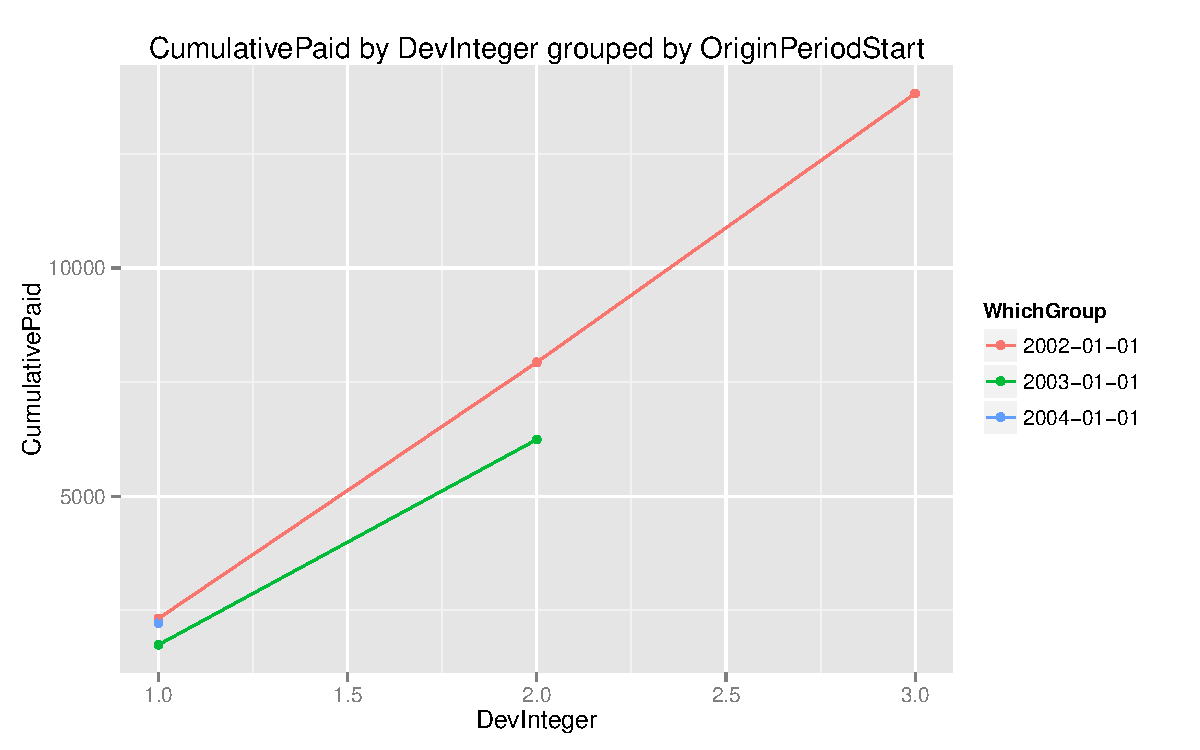
\includegraphics[width=\maxwidth]{figure/VeryBasicExample4} 

\end{knitrout}

\end{frame}

\begin{frame}[fragile]{Something more complex}
\begin{knitrout}
\definecolor{shadecolor}{rgb}{0.969, 0.969, 0.969}\color{fgcolor}\begin{kframe}
\begin{alltt}
\hlfunctioncall{data}(Friedland)
\hlfunctioncall{plotTriangle}(Friedland, Predictor = \hlstring{"DevInteger"}, 
    Response = \hlstring{"CumulativePaid"})
\end{alltt}
\end{kframe}
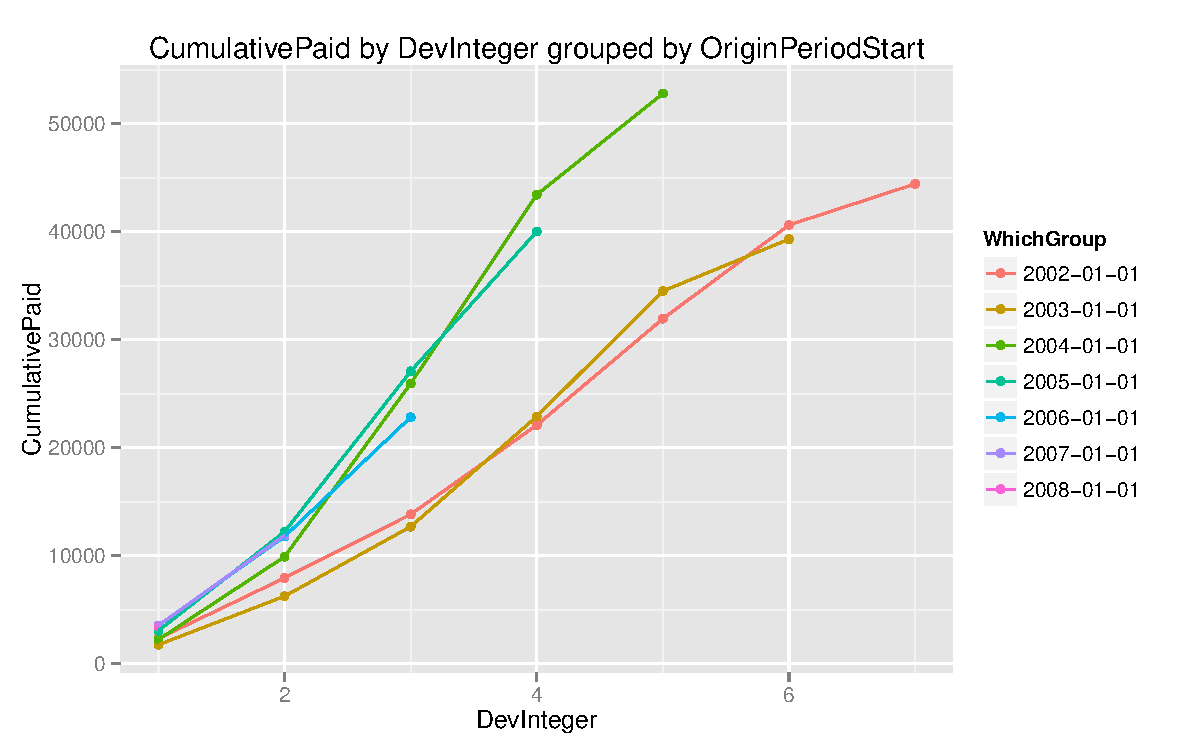
\includegraphics[width=\maxwidth]{figure/Friedland1} 

\end{knitrout}

\end{frame}

\begin{frame}[fragile]{Change the response term}
\begin{knitrout}
\definecolor{shadecolor}{rgb}{0.969, 0.969, 0.969}\color{fgcolor}\begin{kframe}
\begin{alltt}
\hlfunctioncall{plotTriangle}(Friedland, Predictor = \hlstring{"DevInteger"}, 
    Response = \hlstring{"IncrementalPaid"})
\end{alltt}
\end{kframe}
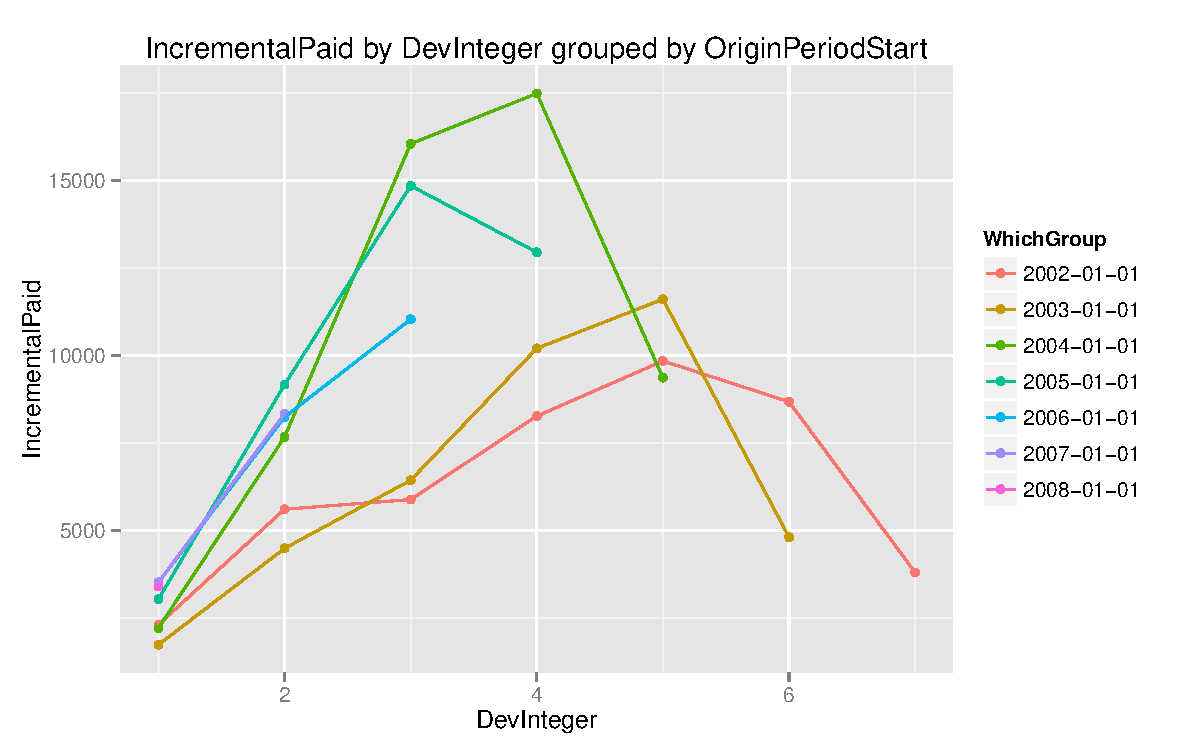
\includegraphics[width=\maxwidth]{figure/Friedland2} 

\end{knitrout}

\end{frame}

\begin{frame}[fragile]{Change the time axis}
\begin{knitrout}
\definecolor{shadecolor}{rgb}{0.969, 0.969, 0.969}\color{fgcolor}\begin{kframe}
\begin{alltt}
\hlfunctioncall{plotTriangle}(Friedland, Predictor = \hlstring{"EvaluationDate"}, 
    Response = \hlstring{"IncrementalPaid"})
\end{alltt}
\end{kframe}
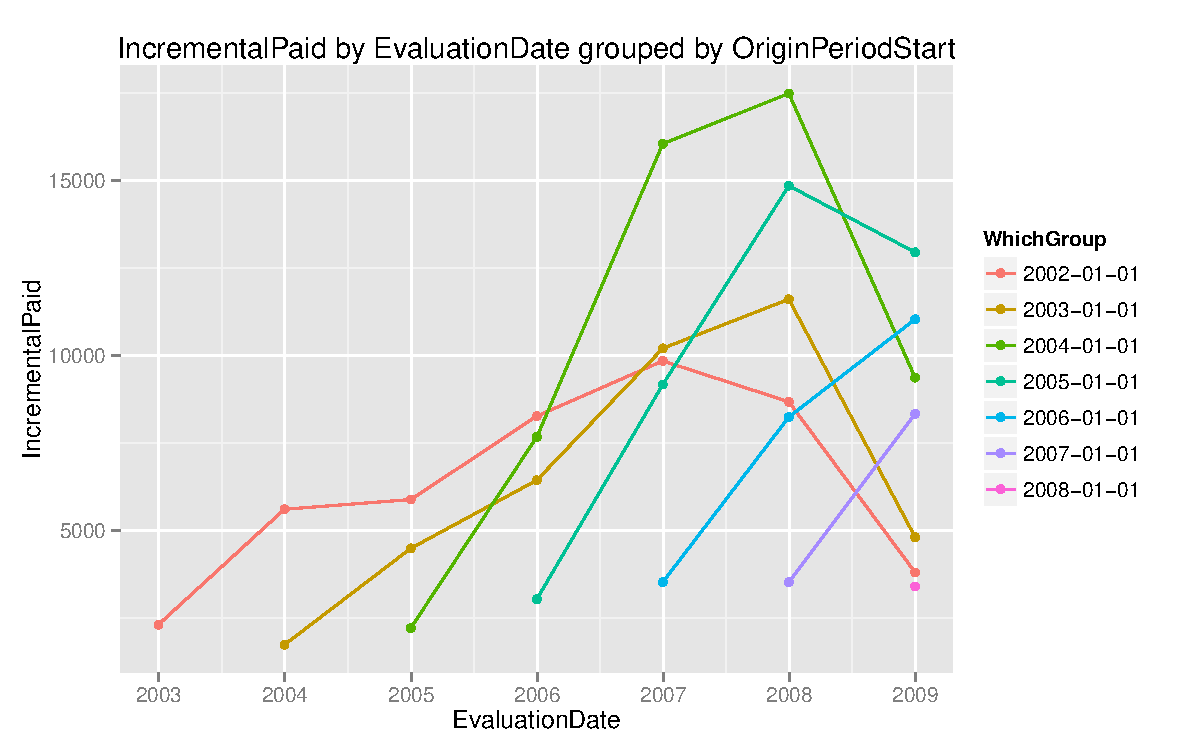
\includegraphics[width=\maxwidth]{figure/Friedland3} 

\end{knitrout}

\end{frame}

\begin{frame}[fragile]{Change the grouping dimension}
\begin{knitrout}
\definecolor{shadecolor}{rgb}{0.969, 0.969, 0.969}\color{fgcolor}\begin{kframe}
\begin{alltt}
\hlfunctioncall{plotTriangle}(Friedland, Predictor = \hlstring{"PriorPaid"}, 
    Response = \hlstring{"IncrementalPaid"}, Group = \hlstring{"DevInteger"}, 
    Lines = FALSE)
\end{alltt}
\end{kframe}
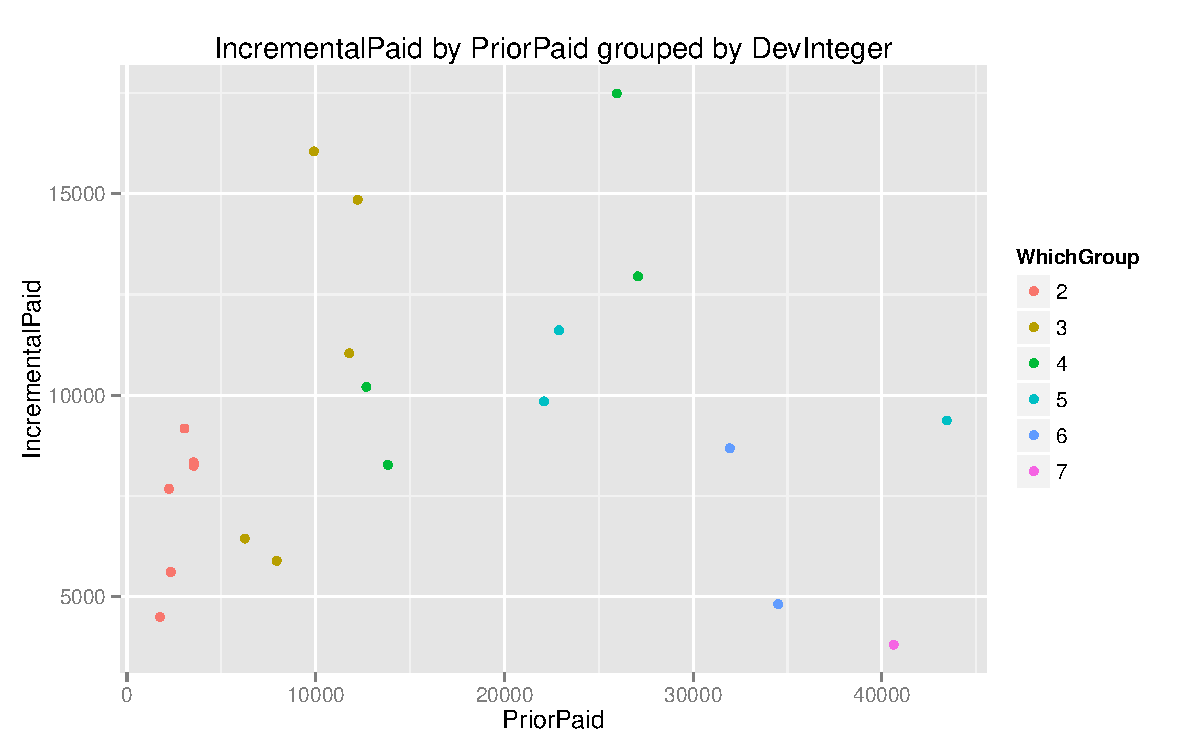
\includegraphics[width=\maxwidth]{figure/FriedlandCL1} 

\end{knitrout}

\end{frame}

\begin{frame}[fragile]{Add fit lines}
\begin{knitrout}
\definecolor{shadecolor}{rgb}{0.969, 0.969, 0.969}\color{fgcolor}\begin{kframe}
\begin{alltt}
\hlfunctioncall{plotTriangle}(Friedland, Predictor = \hlstring{"PriorPaid"}, 
    Response = \hlstring{"IncrementalPaid"}, Group = \hlstring{"DevInteger"}, 
    Lines = FALSE, FitLines = TRUE)
\end{alltt}
\end{kframe}
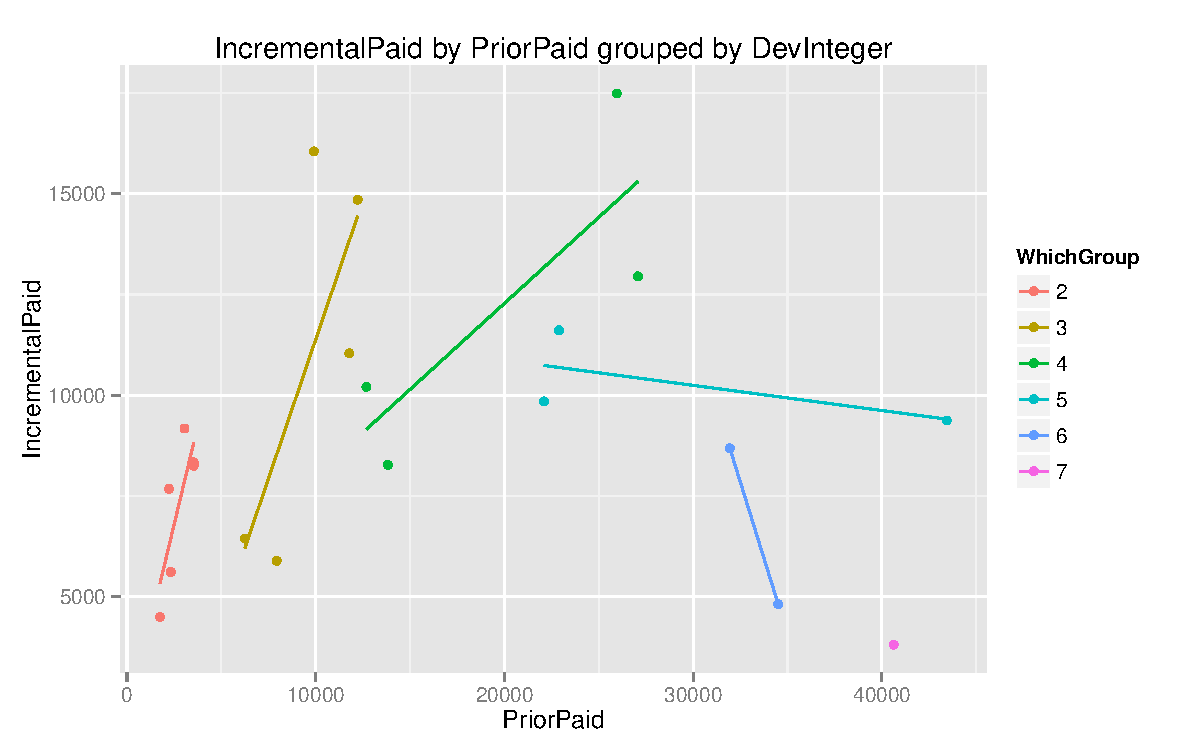
\includegraphics[width=\maxwidth]{figure/Friedland5} 

\end{knitrout}

\end{frame}

\begin{frame}[fragile]{Change the predictor variable}
\begin{knitrout}
\definecolor{shadecolor}{rgb}{0.969, 0.969, 0.969}\color{fgcolor}\begin{kframe}
\begin{alltt}
\hlfunctioncall{plotTriangle}(Friedland, Response = \hlstring{"IncrementalPaid"}, 
    Predictor = \hlstring{"EP"}, Group = \hlstring{"DevInteger"}, 
    Lines = FALSE, FitLines = TRUE)
\end{alltt}
\end{kframe}
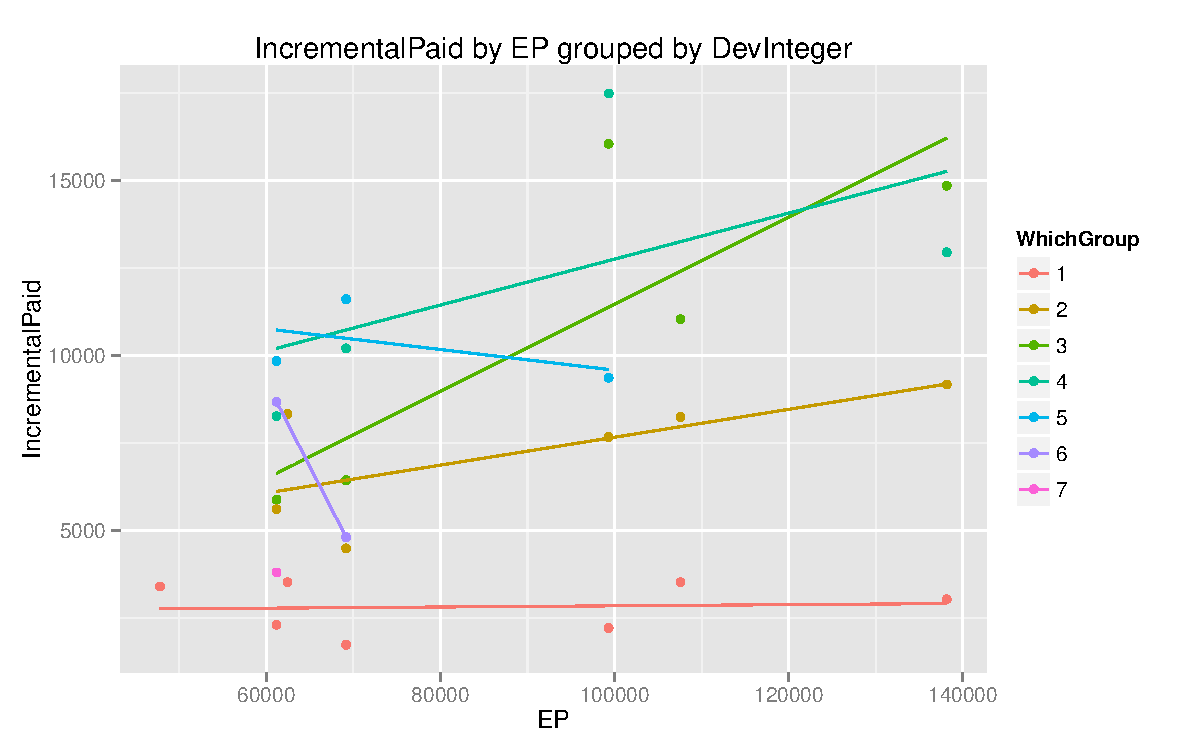
\includegraphics[width=\maxwidth]{figure/Friedland4} 

\end{knitrout}

\end{frame}

\begin{frame}[fragile]{Fit a model}
\begin{knitrout}
\definecolor{shadecolor}{rgb}{0.969, 0.969, 0.969}\color{fgcolor}\begin{kframe}
\begin{alltt}
PaidAM = \hlfunctioncall{newTriangleModel}(Triangle = Friedland, 
    Response = \hlstring{"IncrementalPaid"}, Predictor = \hlstring{"EP"}, 
    FitCategory = \hlstring{"DevInteger"}, Tail = 6)
\end{alltt}
\end{kframe}
\end{knitrout}

\end{frame}

\begin{frame}[fragile]{Visualization is closely related to a model}
\begin{knitrout}
\definecolor{shadecolor}{rgb}{0.969, 0.969, 0.969}\color{fgcolor}\begin{kframe}
\begin{alltt}
\hlfunctioncall{plotTriangle}(Friedland, Response = \hlstring{"IncrementalPaid"}, 
    Predictor = \hlstring{"EP"}, Group = \hlstring{"DevInteger"}, 
    Lines = FALSE, FitLines = TRUE)
PaidAM = \hlfunctioncall{newTriangleModel}(Friedland, Response = \hlstring{"IncrementalPaid"}, 
    Predictor = \hlstring{"EP"}, FitCategory = \hlstring{"DevInteger"}, 
    Tail = 6)
\end{alltt}
\end{kframe}
\end{knitrout}

\end{frame}

\begin{frame}[fragile]{Linear regression in R}
\begin{knitrout}
\definecolor{shadecolor}{rgb}{0.969, 0.969, 0.969}\color{fgcolor}\begin{kframe}
\begin{alltt}
\hlfunctioncall{set.seed}(1234)
N = 100
e = \hlfunctioncall{rnorm}(N, mean = 0, sd = 1)
B0 = 5
B1 = 1.5

X1 = \hlfunctioncall{rep}(\hlfunctioncall{seq}(1, 10), 10)
Y = B0 + B1 * X1 + e

df = \hlfunctioncall{data.frame}(Y = Y, X1 = X1, e = e)
\end{alltt}
\end{kframe}
\end{knitrout}

\end{frame}

\begin{frame}[fragile]{Fitting a linear model}
\begin{knitrout}
\definecolor{shadecolor}{rgb}{0.969, 0.969, 0.969}\color{fgcolor}\begin{kframe}
\begin{alltt}
myFit = \hlfunctioncall{lm}(Y ~ X1, data = df)
\end{alltt}
\end{kframe}
\end{knitrout}

\end{frame}

\begin{frame}[fragile]{Diagnostic output}
\begin{knitrout}\tiny
\definecolor{shadecolor}{rgb}{0.969, 0.969, 0.969}\color{fgcolor}\begin{kframe}
\begin{alltt}
\hlfunctioncall{summary}(myFit)
\end{alltt}
\begin{verbatim}
## 
## Call:
## lm(formula = Y ~ X1, data = df)
## 
## Residuals:
##    Min     1Q Median     3Q    Max 
## -2.188 -0.742 -0.228  0.629  2.709 
## 
## Coefficients:
##             Estimate Std. Error t value
## (Intercept)   4.8383     0.2181    22.2
## X1            1.5009     0.0351    42.7
##             Pr(>|t|)    
## (Intercept)   <2e-16 ***
## X1            <2e-16 ***
## ---
## Signif. codes:  0 '***' 0.001 '**' 0.01 '*' 0.05 '.' 0.1 ' ' 1
## 
## Residual standard error: 1.01 on 98 degrees of freedom
## Multiple R-squared:  0.949,	Adjusted R-squared:  0.948 
## F-statistic: 1.82e+03 on 1 and 98 DF,  p-value: <2e-16
\end{verbatim}
\end{kframe}
\end{knitrout}

\end{frame}

\begin{frame}{Formulas in R}
  \begin{itemize}
    \item The '\textasciitilde' is typically read "is modeled as"
    \item The '+' operator adds new predictor variables to the model
    \item To use operators normally, enclose them in I()
    \item An intercept is always assumed. To remove it, add '+ 0' or '- 1' to the formula
    \item The ':' operator controls interactions between variables.
  \end{itemize}
\end{frame}

\begin{frame}[fragile]{Some examples}
\begin{knitrout}
\definecolor{shadecolor}{rgb}{0.969, 0.969, 0.969}\color{fgcolor}\begin{kframe}
\begin{alltt}
\hlcomment{# The 1 is not necessary}
\hlfunctioncall{lm}(Y ~ 1 + X1, data = df)

\hlcomment{# This is the same as above}
\hlfunctioncall{lm}(Y ~ X1, data = df)

\hlfunctioncall{lm}(Y ~ 0 + X1, data = df)  \hlcomment{#No intercept}

\hlfunctioncall{lm}(Y ~ X1 + X2, data = df)  \hlcomment{#Two predictors}

\hlcomment{# Two predictors and an interaction}
\hlfunctioncall{lm}(Y ~ X1 + X2 + X1:X2, data = df)

\hlcomment{# Use the operators normally}
\hlfunctioncall{lm}(Y ~ \hlfunctioncall{I}(X1/X2), data = df)
\end{alltt}
\end{kframe}
\end{knitrout}

\end{frame}

\begin{frame}[fragile]{Plot the data}
\begin{knitrout}
\definecolor{shadecolor}{rgb}{0.969, 0.969, 0.969}\color{fgcolor}\begin{kframe}
\begin{alltt}
\hlfunctioncall{plot}(df$X1, df$Y, pch = 19)

\hlcomment{# To plot the fit line we can type}
\hlcomment{# either this:}
\hlfunctioncall{abline}(myFit$coefficients[[1]], myFit$coefficients[[2]])

\hlcomment{# Or this:}
\hlfunctioncall{lines}(df$X1, \hlfunctioncall{predict}(myFit))
\end{alltt}
\end{kframe}
\end{knitrout}

\end{frame}

\begin{frame}
\begin{knitrout}
\definecolor{shadecolor}{rgb}{0.969, 0.969, 0.969}\color{fgcolor}
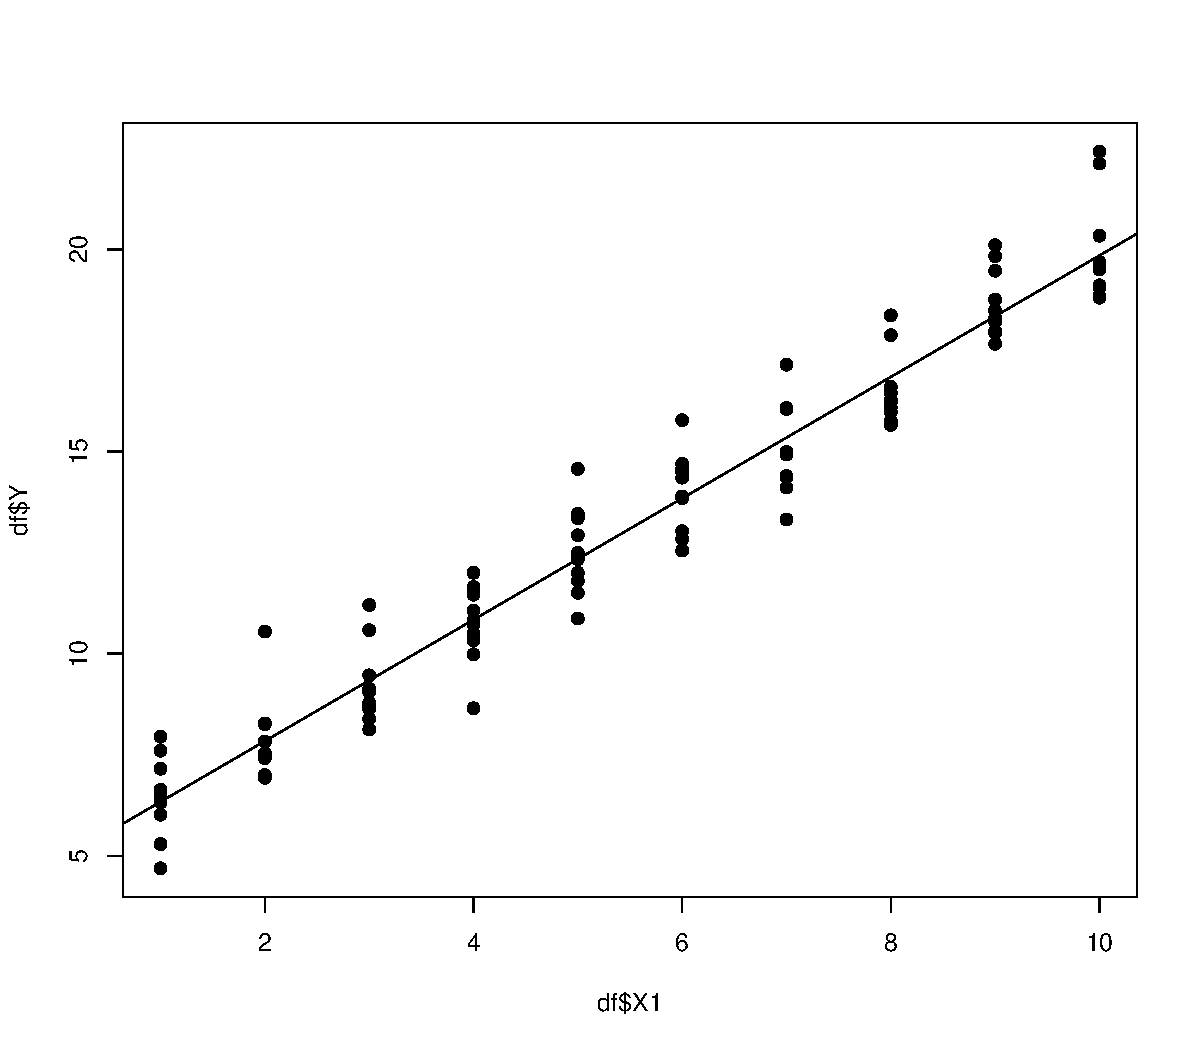
\includegraphics[width=\maxwidth]{figure/UnivariatePlotEval} 

\end{knitrout}

\end{frame}

\begin{frame}[fragile]{More than one variable}
\begin{knitrout}
\definecolor{shadecolor}{rgb}{0.969, 0.969, 0.969}\color{fgcolor}\begin{kframe}
\begin{alltt}
B2 = -3
df$X2 = \hlfunctioncall{rep}(\hlfunctioncall{seq}(-20, -11), 10)
df$Y = \hlfunctioncall{with}(df, B0 + B1 * X1 + B2 * X2)
myFit2 = \hlfunctioncall{lm}(Y ~ X1 + X2, data = df)
\end{alltt}
\end{kframe}
\end{knitrout}

How would we plot this data?
\end{frame}

\begin{frame}[fragile]{A spurious variable}
\begin{knitrout}
\definecolor{shadecolor}{rgb}{0.969, 0.969, 0.969}\color{fgcolor}\begin{kframe}
\begin{alltt}
df$spurious = \hlfunctioncall{runif}(N, min = -5, max = 5)
myFit3 = \hlfunctioncall{lm}(Y ~ X1 + spurious, data = df)
\end{alltt}
\end{kframe}
\end{knitrout}

How would you determine whether or not to include the spurious predictor?
\end{frame}

\begin{frame}[fragile]{Linear regression assumptions}
  \begin{enumerate}
    \item Linear model with specified parameters
      \begin{itemize}
        \item Significance of individual model factors
        \item Significance of model
      \end{itemize}
    \item Functional form of errors
    \item Independence of errors
      \begin{itemize}
        \item (Serial) correlation of errors
        \item Homoskedasticity
      \end{itemize}
  \end{enumerate}
\end{frame}

\begin{frame}[fragile]{Linear regression assumptions}
  \begin{enumerate}
    \item Linear model with specified parameters
      \begin{itemize}
        \item \color{blue} Significance of individual model factors
        \item Significance of model
      \end{itemize}
    \item Functional form of errors
    \item Independence of errors
      \begin{itemize}
        \item (Serial) correlation of errors
        \item Homoskedasticity
      \end{itemize}
  \end{enumerate}
\end{frame}

\begin{frame}[fragile]{Significance of model factors}
  Each model factor follows a t distribution, whose parameters depends on the underlying data. The "t value" reported by R is the ratio of the mean to the standard error. As a simple rule of thumb, any time a t-stat divided by its standard error is less than 2, one should reevaluate whether that factor improves the overall model. Put differently, such a low "t value" makes it difficult to reject the null hypothesis that the mean of the model factor is zero.
\end{frame}

\begin{frame}[fragile]{Significance of model factors (cont'd)}
\begin{knitrout}\tiny
\definecolor{shadecolor}{rgb}{0.969, 0.969, 0.969}\color{fgcolor}\begin{kframe}
\begin{alltt}
dfCoef = \hlfunctioncall{summary}(myFit)$coefficients
dfCoef
\end{alltt}
\begin{verbatim}
##             Estimate Std. Error t value
## (Intercept)    4.838    0.21808   22.19
## X1             1.501    0.03515   42.70
##              Pr(>|t|)
## (Intercept) 5.423e-40
## X1          3.863e-65
\end{verbatim}
\end{kframe}
\end{knitrout}

\end{frame}

\begin{frame}[fragile]{Significance of model factors (cont'd)}
\begin{knitrout}\tiny
\definecolor{shadecolor}{rgb}{0.969, 0.969, 0.969}\color{fgcolor}\begin{kframe}
\begin{alltt}
spuriousFit = \hlfunctioncall{lm}(Y ~ spurious, data = df)
dfCoef = \hlfunctioncall{summary}(spuriousFit)$coefficients
dfCoef
\end{alltt}
\begin{verbatim}
##             Estimate Std. Error t value
## (Intercept)  59.7520     0.4328 138.052
## spurious     -0.1712     0.1640  -1.044
##               Pr(>|t|)
## (Intercept) 4.395e-114
## spurious     2.992e-01
\end{verbatim}
\end{kframe}
\end{knitrout}

\end{frame}

\begin{frame}[fragile]{Two different reserving models}
\begin{knitrout}
\definecolor{shadecolor}{rgb}{0.969, 0.969, 0.969}\color{fgcolor}\begin{kframe}
\begin{alltt}
PaidCL = \hlfunctioncall{newTriangleModel}(Friedland, Response = \hlstring{"IncrementalPaid"}, 
    Predictor = \hlstring{"PriorPaid"}, FitCategory = \hlstring{"DevInteger"}, 
    Tail = 6)
PaidAM = \hlfunctioncall{newTriangleModel}(Triangle = Friedland, 
    Response = \hlstring{"IncrementalPaid"}, Predictor = \hlstring{"EP"}, 
    FitCategory = \hlstring{"DevInteger"}, Tail = 6)
\end{alltt}
\end{kframe}
\end{knitrout}

The first model corresponds to the traditional multiplicative chain ladder as applied to paid losses. The default is to have no weighting.
\newline The second model is the additive model. This is described in Stanard and elsewhere.
\end{frame}

\begin{frame}[fragile]
\begin{knitrout}\tiny
\definecolor{shadecolor}{rgb}{0.969, 0.969, 0.969}\color{fgcolor}\begin{kframe}
\begin{alltt}
\hlfunctioncall{summary}(PaidCL@Fit)$coefficients[, 1:2]
\end{alltt}
\begin{verbatim}
##                           Estimate
## PriorPaid:FitCategory2      2.6167
## PriorPaid:FitCategory3      1.1425
## PriorPaid:FitCategory4      0.5962
## PriorPaid:FitCategory5      0.3072
## PriorPaid:FitCategoryTail   0.1549
##                           Std. Error
## PriorPaid:FitCategory2       0.42044
## PriorPaid:FitCategory3       0.13123
## PriorPaid:FitCategory4       0.06912
## PriorPaid:FitCategory5       0.05383
## PriorPaid:FitCategoryTail    0.04664
\end{verbatim}
\end{kframe}
\end{knitrout}

\end{frame}

\begin{frame}[fragile]{Observe the model factors - Chain Ladder}
\begin{knitrout}
\definecolor{shadecolor}{rgb}{0.969, 0.969, 0.969}\color{fgcolor}\begin{kframe}
\begin{alltt}
\hlfunctioncall{PlotModelFactors}(PaidCL)
\end{alltt}
\end{kframe}
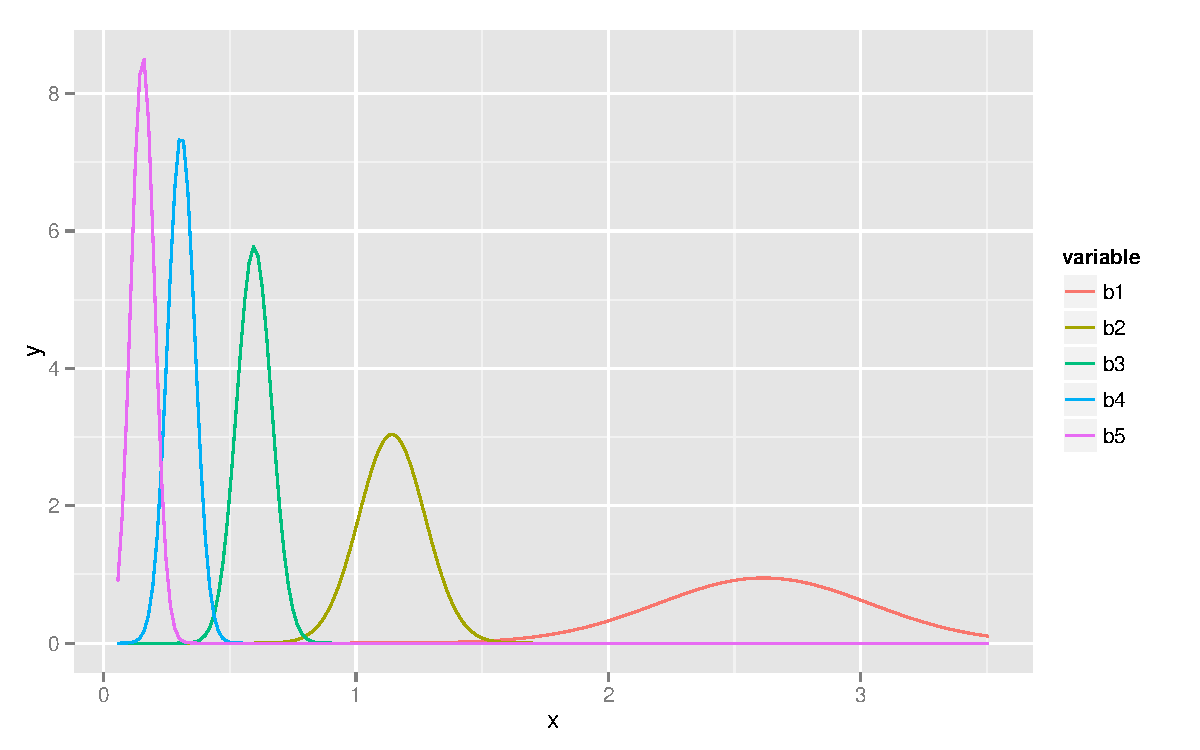
\includegraphics[width=\maxwidth]{figure/PlotModelFactorsCL} 

\end{knitrout}

\end{frame}

\begin{frame}[fragile]{Observe the model factors - Additive}
\begin{knitrout}
\definecolor{shadecolor}{rgb}{0.969, 0.969, 0.969}\color{fgcolor}\begin{kframe}
\begin{alltt}
\hlfunctioncall{PlotModelFactors}(PaidAM)
\end{alltt}
\end{kframe}
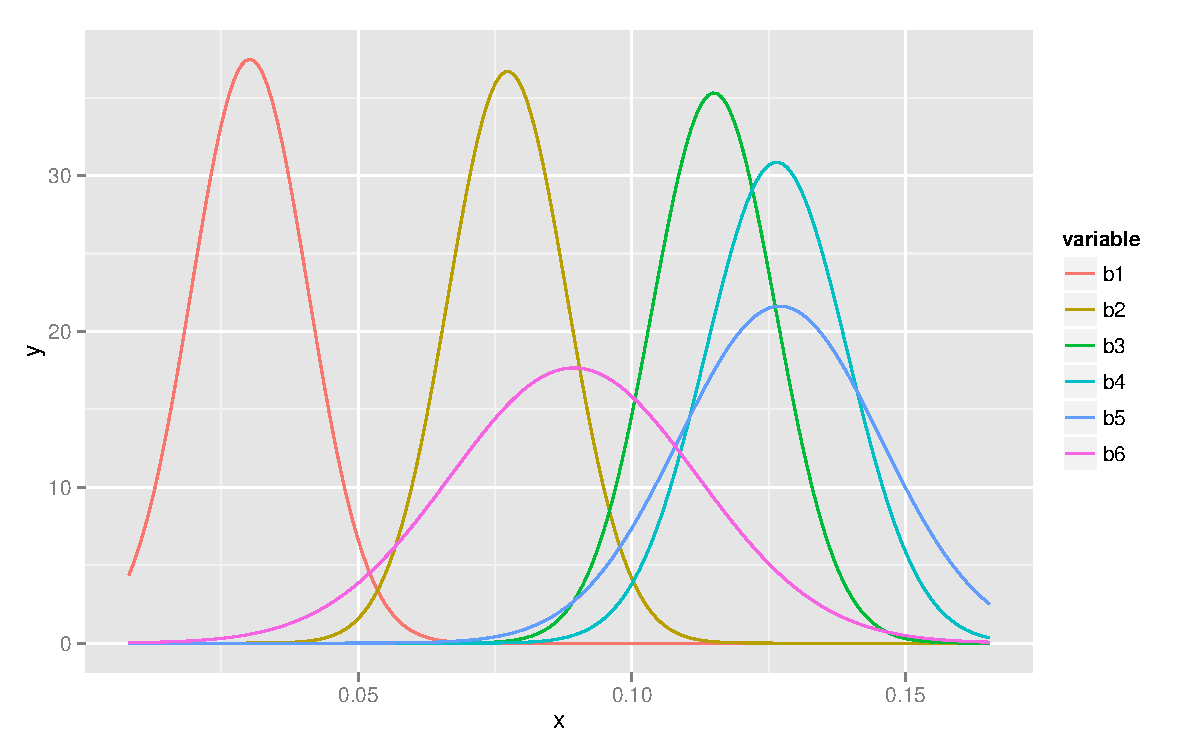
\includegraphics[width=\maxwidth]{figure/PlotModelFactorsAM} 

\end{knitrout}

\end{frame}

\begin{frame}[fragile]{Linear regression assumptions}
  \begin{enumerate}
    \item Linear model with specified parameters
      \begin{itemize}
        \item Significance of individual model factors
        \item \color{blue} Significance of model
      \end{itemize}
    \item Functional form of errors
    \item Independence of errors
      \begin{itemize}
        \item (Serial) correlation of errors
        \item Homoskedasticity
      \end{itemize}
  \end{enumerate}
\end{frame}

\begin{frame}[fragile]{Significance of model}
  Several metrics
  \begin{enumerate}
    \item R-squared
    \item F-statistic
    \item AIC
    \item Penalized measures
  \end{enumerate}
\end{frame}

\begin{frame}[fragile]{Diagnostics}
\begin{knitrout}
\definecolor{shadecolor}{rgb}{0.969, 0.969, 0.969}\color{fgcolor}\begin{kframe}
\begin{alltt}
\hlfunctioncall{summary}(myFit)$r.squared
\end{alltt}
\begin{verbatim}
## [1] 0.949
\end{verbatim}
\begin{alltt}
\hlfunctioncall{summary}(myFit)$fstatistic
\end{alltt}
\begin{verbatim}
## value numdf dendf 
##  1824     1    98
\end{verbatim}
\end{kframe}
\end{knitrout}

Be careful of both of these statistics. Always visualize your data!
\end{frame}

\begin{frame}[fragile]{The F stat distribution looks good}
\begin{knitrout}
\definecolor{shadecolor}{rgb}{0.969, 0.969, 0.969}\color{fgcolor}\begin{kframe}
\begin{alltt}
\hlfunctioncall{PlotModelGoF}(PaidAM)
\end{alltt}
\end{kframe}
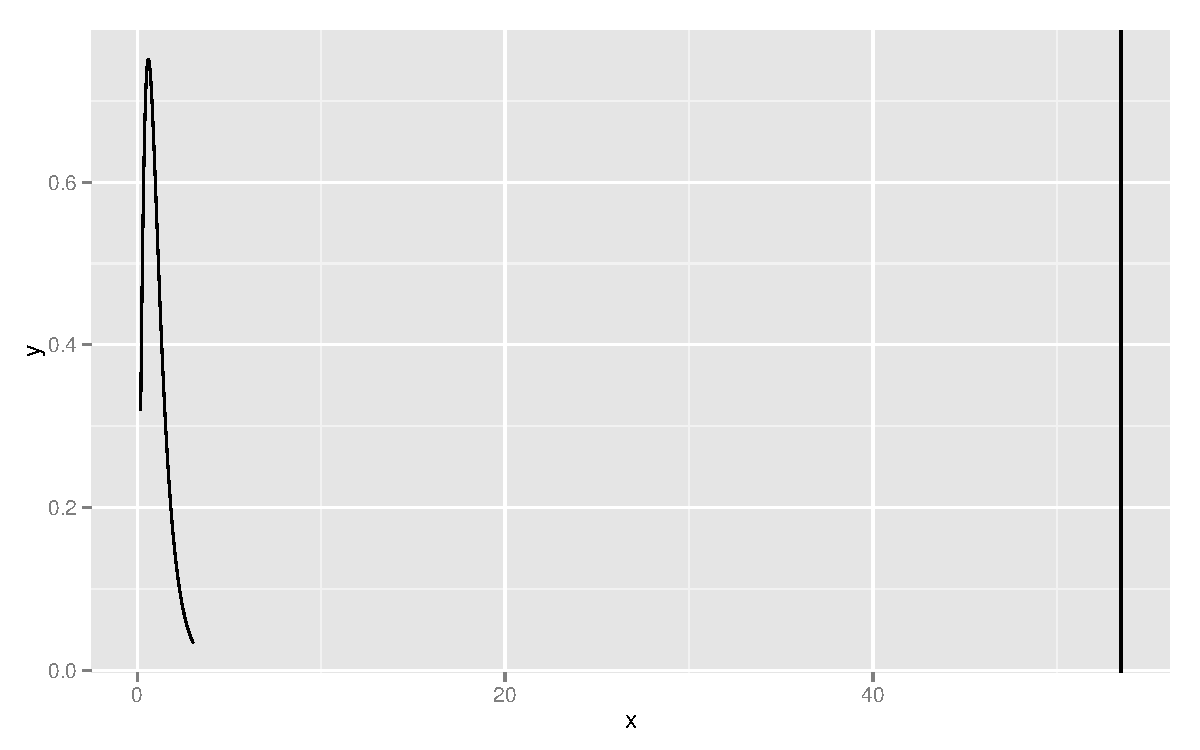
\includegraphics[width=\maxwidth]{figure/PaidCLGoF} 

\end{knitrout}

\end{frame}

\begin{frame}[fragile]{But always observe the residual plots!}
\begin{knitrout}
\definecolor{shadecolor}{rgb}{0.969, 0.969, 0.969}\color{fgcolor}\begin{kframe}
\begin{alltt}
\hlfunctioncall{PlotResiduals}(PaidAM)
\end{alltt}
\end{kframe}
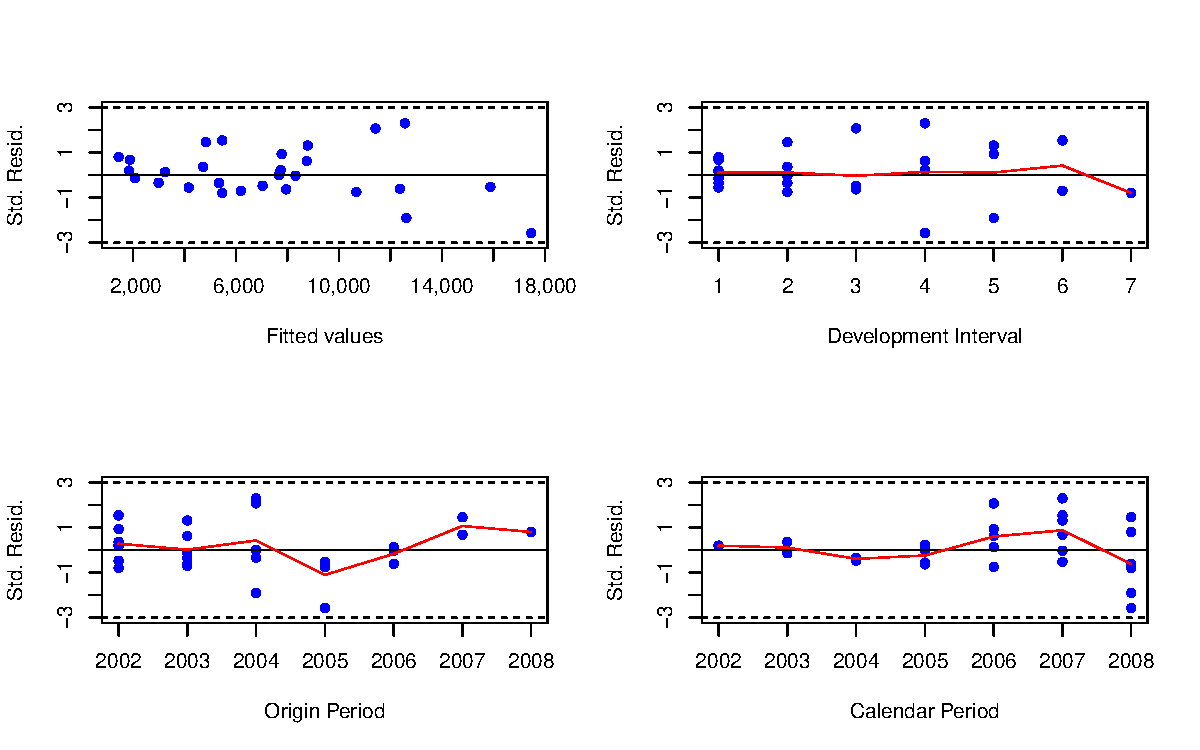
\includegraphics[width=\maxwidth]{figure/ResidualPlotsAM} 

\end{knitrout}

\end{frame}

\begin{frame}[fragile]{Your turn}
\begin{knitrout}
\definecolor{shadecolor}{rgb}{0.969, 0.969, 0.969}\color{fgcolor}\begin{kframe}
\begin{alltt}
\hlfunctioncall{head}(df)
\end{alltt}
\begin{verbatim}
##      Y X1       e  X2 spurious
## 1 66.5  1 -1.2071 -20   1.6075
## 2 65.0  2  0.2774 -19   0.2836
## 3 63.5  3  1.0844 -18  -1.8251
## 4 62.0  4 -2.3457 -17   2.6786
## 5 60.5  5  0.4291 -16   0.2631
## 6 59.0  6  0.5061 -15   2.3230
\end{verbatim}
\end{kframe}
\end{knitrout}

Fit a linear model with and without X1 and X2. Which model fits better? How would you determine whether to include the spurious parameter?
\end{frame}

\begin{frame}[fragile]{Linear regression assumptions}
  \begin{enumerate}
    \item Linear model with specified parameters
      \begin{itemize}
        \item Significance of individual model factors
        \item Significance of model
      \end{itemize}
    \item \color{blue} Functional form of errors
    \item \color{black} Independence of errors
      \begin{itemize}
        \item (Serial) correlation of errors
        \item Homoskedasticity
      \end{itemize}
  \end{enumerate}
\end{frame}

\begin{frame}[fragile]{Test for normalcy}
\begin{knitrout}
\definecolor{shadecolor}{rgb}{0.969, 0.969, 0.969}\color{fgcolor}\begin{kframe}
\begin{alltt}
\hlfunctioncall{shapiro.test}(e)
\end{alltt}
\begin{verbatim}
## 
## 	Shapiro-Wilk normality test
## 
## data:  e
## W = 0.9659, p-value = 0.01078
\end{verbatim}
\end{kframe}
\end{knitrout}

\begin{knitrout}
\definecolor{shadecolor}{rgb}{0.969, 0.969, 0.969}\color{fgcolor}\begin{kframe}
\begin{alltt}
\hlfunctioncall{qqnorm}(e)
\hlfunctioncall{qqline}(e)
\end{alltt}
\end{kframe}
\end{knitrout}

\end{frame}

\begin{frame}[fragile]
\begin{knitrout}
\definecolor{shadecolor}{rgb}{0.969, 0.969, 0.969}\color{fgcolor}
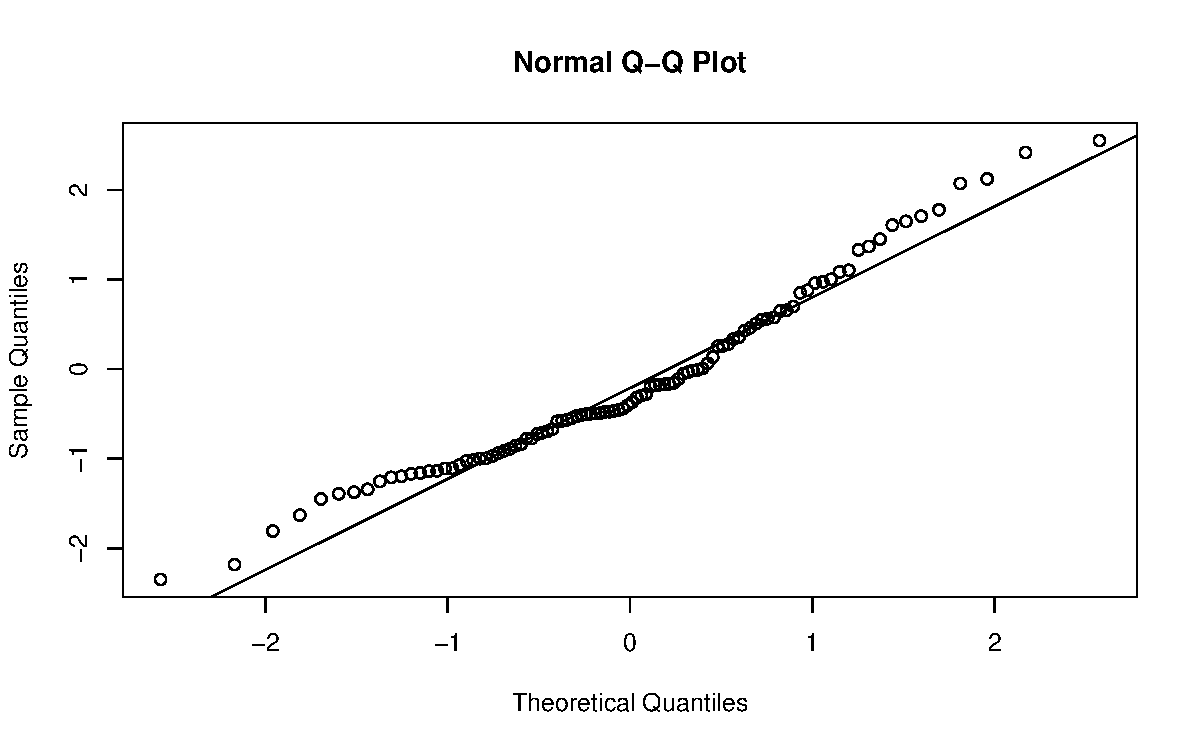
\includegraphics[width=\maxwidth]{figure/ShapiroWilkPlot2} 

\end{knitrout}

\end{frame}

\begin{frame}[fragile]{Linear regression assumptions}
  \begin{enumerate}
    \item Linear model with specified parameters
      \begin{itemize}
        \item Significance of individual model factors
        \item Significance of model
      \end{itemize}
    \item Functional form of errors
    \item Independence of errors
      \begin{itemize}
        \item \color{blue} (Serial) correlation of errors
        \item \color{black} Homoskedasticity
      \end{itemize}
  \end{enumerate}
\end{frame}

\begin{frame}[fragile]{Error correlation}
\begin{knitrout}
\definecolor{shadecolor}{rgb}{0.969, 0.969, 0.969}\color{fgcolor}\begin{kframe}
\begin{alltt}
lstFitResults = \hlfunctioncall{plotSerialCorrelation}(PaidAM)
\end{alltt}
\end{kframe}
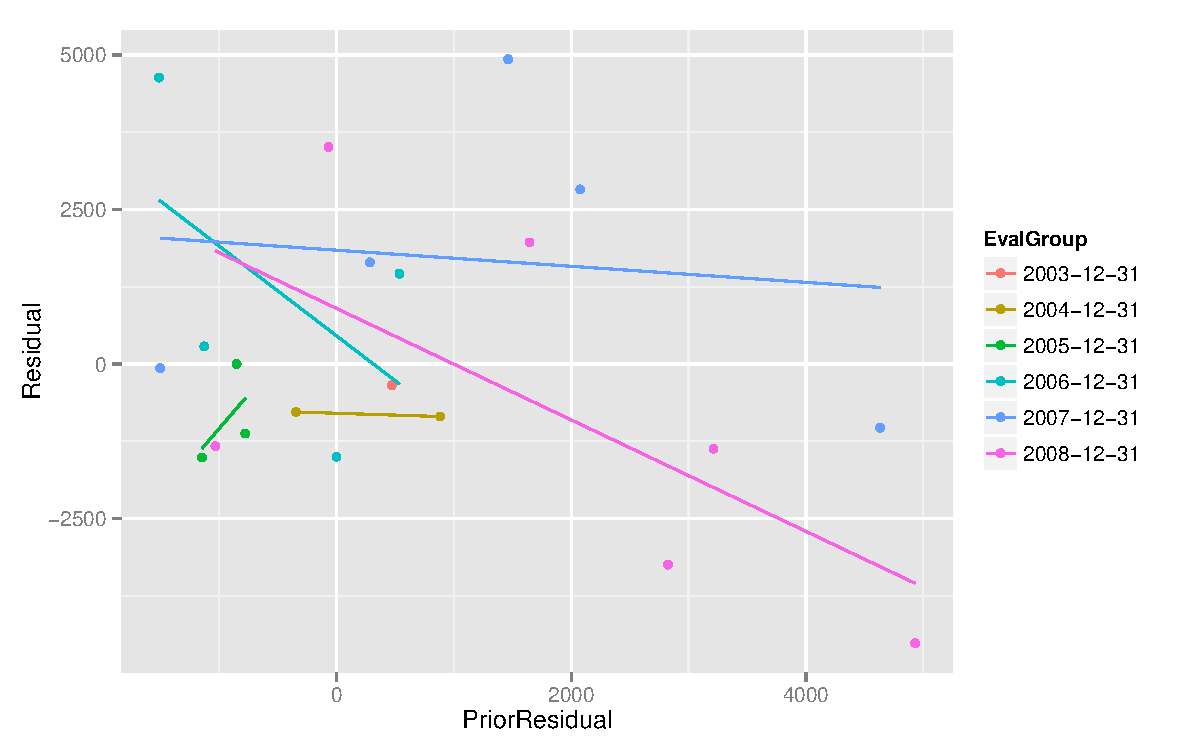
\includegraphics[width=\maxwidth]{figure/SerialCorrelationPlot} 

\end{knitrout}

\end{frame}

\begin{frame}[fragile]{Error summary}
\begin{knitrout}\tiny
\definecolor{shadecolor}{rgb}{0.969, 0.969, 0.969}\color{fgcolor}\begin{kframe}
\begin{alltt}
\hlfunctioncall{summary}(lstFitResults$fit)$coefficients
\end{alltt}
\begin{verbatim}
##                                   Estimate
## PriorResidual:EvalGroup2003-12-31  -0.7290
## PriorResidual:EvalGroup2004-12-31  -0.5376
## PriorResidual:EvalGroup2005-12-31   0.9879
## PriorResidual:EvalGroup2006-12-31  -1.7029
## PriorResidual:EvalGroup2007-12-31   0.2934
## PriorResidual:EvalGroup2008-12-31  -0.6783
##                                   Std. Error
## PriorResidual:EvalGroup2003-12-31     4.8838
## PriorResidual:EvalGroup2004-12-31     2.4270
## PriorResidual:EvalGroup2005-12-31     1.4203
## PriorResidual:EvalGroup2006-12-31     1.1767
## PriorResidual:EvalGroup2007-12-31     0.4192
## PriorResidual:EvalGroup2008-12-31     0.3385
##                                   t value
## PriorResidual:EvalGroup2003-12-31 -0.1493
## PriorResidual:EvalGroup2004-12-31 -0.2215
## PriorResidual:EvalGroup2005-12-31  0.6956
## PriorResidual:EvalGroup2006-12-31 -1.4471
## PriorResidual:EvalGroup2007-12-31  0.6998
## PriorResidual:EvalGroup2008-12-31 -2.0041
##                                   Pr(>|t|)
## PriorResidual:EvalGroup2003-12-31  0.88333
## PriorResidual:EvalGroup2004-12-31  0.82768
## PriorResidual:EvalGroup2005-12-31  0.49733
## PriorResidual:EvalGroup2006-12-31  0.16845
## PriorResidual:EvalGroup2007-12-31  0.49475
## PriorResidual:EvalGroup2008-12-31  0.06346
\end{verbatim}
\end{kframe}
\end{knitrout}

\end{frame}

\begin{frame}[fragile]{Introduce correlation}
\begin{knitrout}
\definecolor{shadecolor}{rgb}{0.969, 0.969, 0.969}\color{fgcolor}\begin{kframe}
\begin{alltt}
df = Friedland@TriangleData
cy = (\hlfunctioncall{year}(df$EvaluationDate) == 2008)
df$IncrementalPaid[cy] = df$IncrementalPaid[cy] * 
    (2/3)

myTriangle = \hlfunctioncall{newTriangle}(df, OriginPeriods = OriginPeriod, 
    DevelopmentLags = DevelopmentLag, StaticMeasures = \hlstring{"EP"}, 
    StochasticMeasures = \hlstring{"IncrementalPaid"}, 
    Cumulative = FALSE)
\end{alltt}


{\ttfamily\noindent\itshape\color{messagecolor}{\#\# estimate only: convert to intervals for accuracy}}\begin{alltt}

myModel = \hlfunctioncall{newTriangleModel}(myTriangle, \hlstring{"IncrementalPaid"}, 
    \hlstring{"EP"}, \hlstring{"DevInteger"})
\end{alltt}
\end{kframe}
\end{knitrout}

\end{frame}

\begin{frame}[fragile]{Error summary}
\begin{knitrout}\tiny
\definecolor{shadecolor}{rgb}{0.969, 0.969, 0.969}\color{fgcolor}\begin{kframe}
\begin{alltt}
lstResult = \hlfunctioncall{FitSerialCorrelation}(myModel)
\hlfunctioncall{summary}(lstResult$fit)$coefficients
\end{alltt}
\begin{verbatim}
##                                   Estimate
## PriorResidual:EvalGroup2003-12-31  -0.5188
## PriorResidual:EvalGroup2004-12-31  -0.3895
## PriorResidual:EvalGroup2005-12-31   0.8558
## PriorResidual:EvalGroup2006-12-31  -0.4754
## PriorResidual:EvalGroup2007-12-31   0.6366
## PriorResidual:EvalGroup2008-12-31  -0.8712
##                                   Std. Error
## PriorResidual:EvalGroup2003-12-31     5.0708
## PriorResidual:EvalGroup2004-12-31     2.4087
## PriorResidual:EvalGroup2005-12-31     2.3931
## PriorResidual:EvalGroup2006-12-31     1.3052
## PriorResidual:EvalGroup2007-12-31     0.3936
## PriorResidual:EvalGroup2008-12-31     0.3044
##                                   t value
## PriorResidual:EvalGroup2003-12-31 -0.1023
## PriorResidual:EvalGroup2004-12-31 -0.1617
## PriorResidual:EvalGroup2005-12-31  0.3576
## PriorResidual:EvalGroup2006-12-31 -0.3643
## PriorResidual:EvalGroup2007-12-31  1.6173
## PriorResidual:EvalGroup2008-12-31 -2.8618
##                                   Pr(>|t|)
## PriorResidual:EvalGroup2003-12-31  0.91987
## PriorResidual:EvalGroup2004-12-31  0.87369
## PriorResidual:EvalGroup2005-12-31  0.72562
## PriorResidual:EvalGroup2006-12-31  0.72074
## PriorResidual:EvalGroup2007-12-31  0.12664
## PriorResidual:EvalGroup2008-12-31  0.01188
\end{verbatim}
\end{kframe}
\end{knitrout}

\end{frame}

\begin{frame}[fragile]{Linear regression assumptions}
  \begin{enumerate}
    \item Linear model with specified parameters
      \begin{itemize}
        \item Significance of individual model factors
        \item Significance of model
      \end{itemize}
    \item Functional form of errors
    \item Independence of errors
      \begin{itemize}
        \item (Serial) correlation of errors
        \item \color{blue} Homoskedasticity
      \end{itemize}
  \end{enumerate}
\end{frame}

\begin{frame}[fragile]{Breusch-Pagan}
Heteroskedasticity is most often detected by observing the residuals. Adjusting the weights of the regression is an implicit assumption about the variance of the response variable. Changing the alpha parameter allows one to adjust for presumed heteroskedasticity. Read papers by Dan Murphy (or just ask him, he's probably standing somewhere close by) to learn more.
\newline There is a formal test from Breusch and Pagan, which is available from the lmtest package.
\end{frame}

\begin{frame}[fragile]
\begin{knitrout}
\definecolor{shadecolor}{rgb}{0.969, 0.969, 0.969}\color{fgcolor}\begin{kframe}
\begin{alltt}
\hlfunctioncall{set.seed}(1234)
N = 100
e = \hlfunctioncall{rnorm}(N, mean = 0, sd = 1)
B1 = 1.5
X1 = \hlfunctioncall{rep}(\hlfunctioncall{seq}(1, 10), 10)
Y = B1 * X1 + \hlfunctioncall{sqrt}(X1) * e

bpFit = \hlfunctioncall{lm}(Y ~ 0 + X1)
\hlfunctioncall{bptest}(bpFit)
\end{alltt}
\begin{verbatim}
## 
## 	studentized Breusch-Pagan test
## 
## data:  bpFit
## BP = 2.64, df = 0, p-value <
## 2.2e-16
\end{verbatim}
\begin{alltt}
\hlfunctioncall{coef}(bpFit)
\end{alltt}
\begin{verbatim}
##    X1 
## 1.445
\end{verbatim}
\end{kframe}
\end{knitrout}

\begin{knitrout}
\definecolor{shadecolor}{rgb}{0.969, 0.969, 0.969}\color{fgcolor}\begin{kframe}
\begin{alltt}
\hlfunctioncall{plot}(X1, \hlfunctioncall{residuals}(bpFit), pch = 19)
\end{alltt}
\end{kframe}
\end{knitrout}

\end{frame}

\begin{frame}[fragile]
\begin{knitrout}
\definecolor{shadecolor}{rgb}{0.969, 0.969, 0.969}\color{fgcolor}
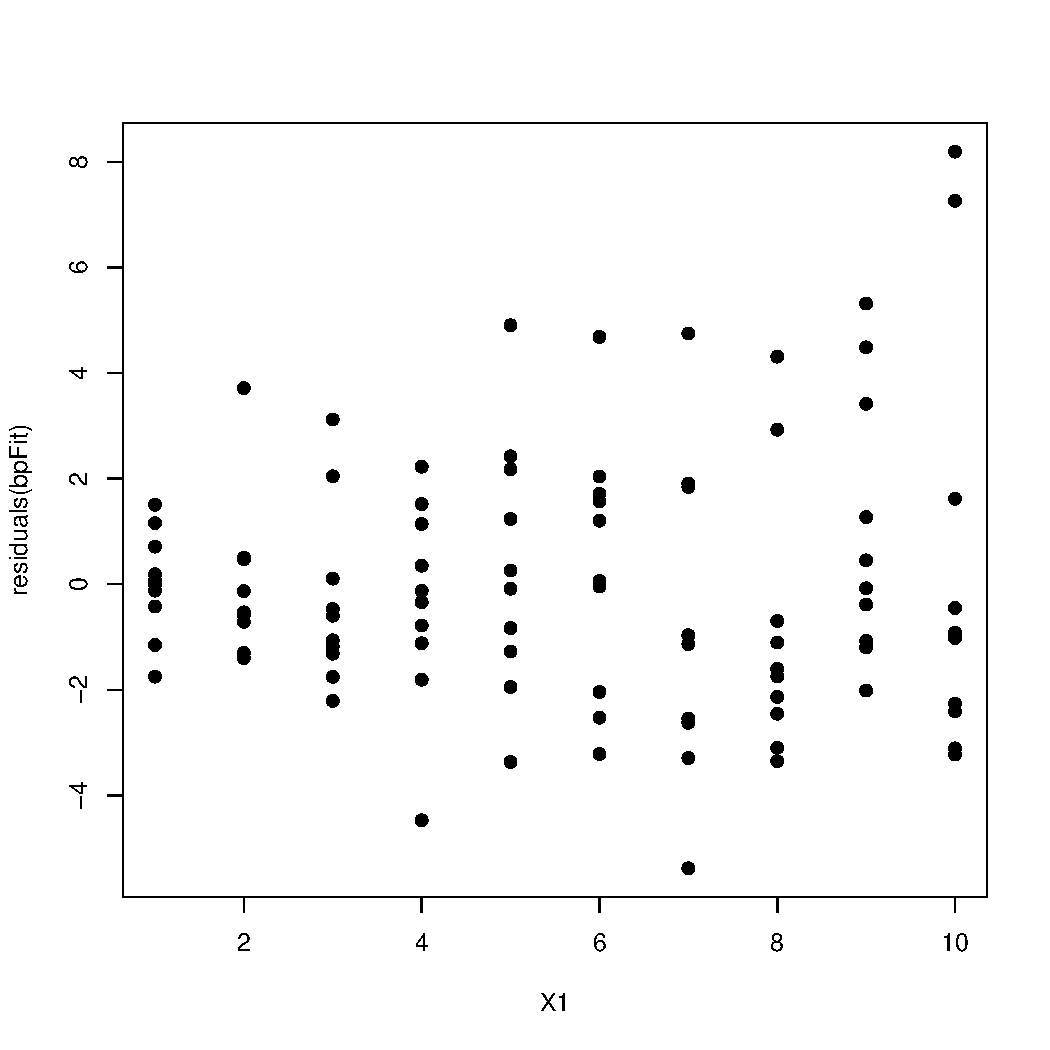
\includegraphics[width=\maxwidth]{figure/BrueschPaganPlot} 

\end{knitrout}

\end{frame}

\begin{frame}[fragile]
\begin{knitrout}
\definecolor{shadecolor}{rgb}{0.969, 0.969, 0.969}\color{fgcolor}\begin{kframe}
\begin{alltt}
alpha = \hlfunctioncall{seq}(-10, 10, by = 0.05)
slope = \hlfunctioncall{sapply}(alpha, \hlfunctioncall{function}(x) \{
    w = X1^x
    fit = \hlfunctioncall{lm}(Y ~ 0 + X1, weight = w)
    \hlfunctioncall{coef}(fit)
\})
\hlfunctioncall{max}(Y/X1)
\end{alltt}
\begin{verbatim}
## [1] 3.302
\end{verbatim}
\begin{alltt}
\hlfunctioncall{min}(Y/X1)
\end{alltt}
\begin{verbatim}
## [1] -0.306
\end{verbatim}
\begin{alltt}
\hlfunctioncall{max}(slope)
\end{alltt}
\begin{verbatim}
## [1] 1.488
\end{verbatim}
\begin{alltt}
\hlfunctioncall{min}(slope)
\end{alltt}
\begin{verbatim}
## [1] 1.425
\end{verbatim}
\end{kframe}
\end{knitrout}

\begin{knitrout}
\definecolor{shadecolor}{rgb}{0.969, 0.969, 0.969}\color{fgcolor}\begin{kframe}
\begin{alltt}
\hlfunctioncall{plot}(alpha, slope, pch = 19)
\end{alltt}
\end{kframe}
\end{knitrout}

\end{frame}

\begin{frame}[fragile]
\begin{knitrout}
\definecolor{shadecolor}{rgb}{0.969, 0.969, 0.969}\color{fgcolor}
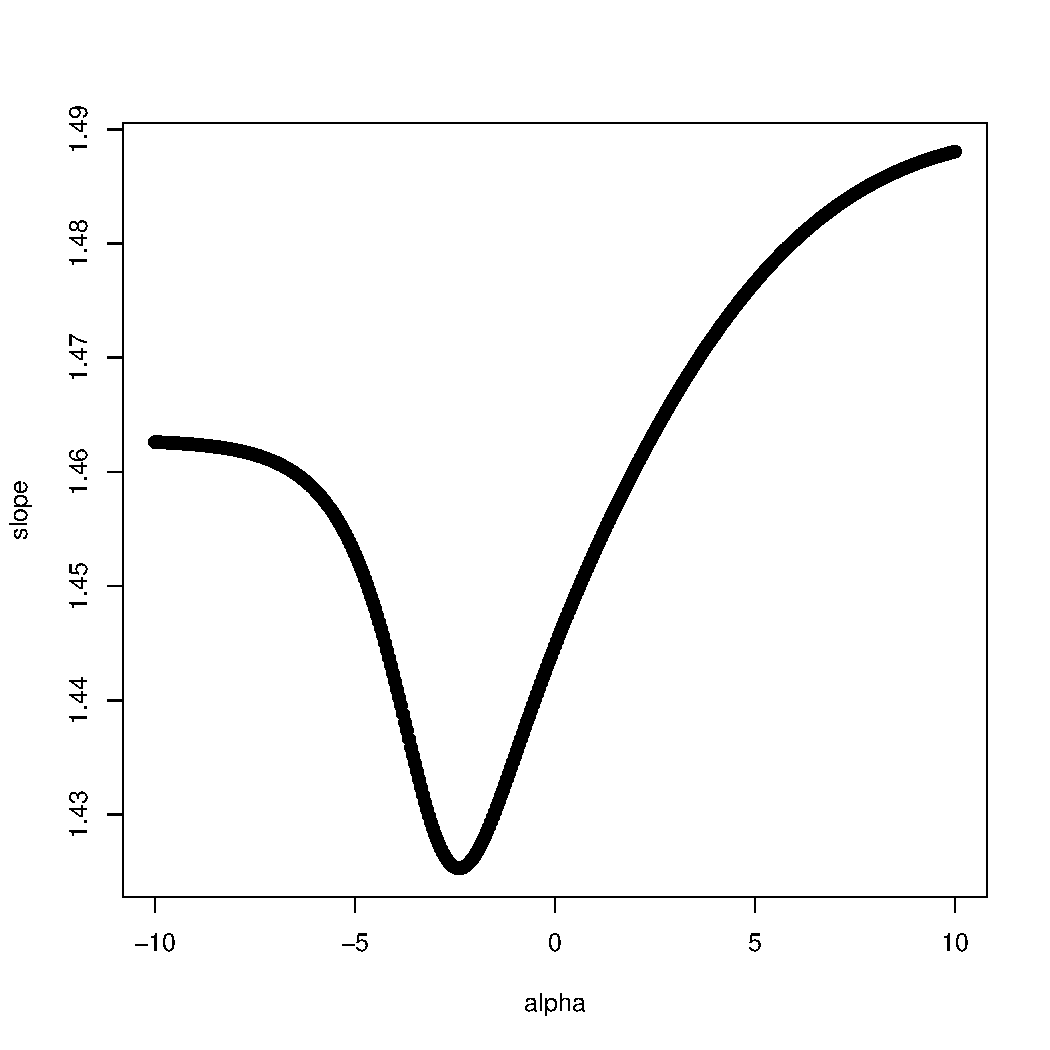
\includegraphics[width=\maxwidth]{figure/unnamed-chunk-6} 

\end{knitrout}

\end{frame}

\begin{frame}[fragile]
\begin{knitrout}
\definecolor{shadecolor}{rgb}{0.969, 0.969, 0.969}\color{fgcolor}\begin{kframe}
\begin{alltt}
\hlfunctioncall{plot}(X1, Y, pch = 19)
\hlfunctioncall{abline}(0, \hlfunctioncall{min}(slope), col = \hlstring{"blue"})
\hlfunctioncall{abline}(0, \hlfunctioncall{max}(slope), col = \hlstring{"blue"})
\hlfunctioncall{abline}(0, B1, col = \hlstring{"red"})
\end{alltt}
\end{kframe}
\end{knitrout}

\end{frame}

\begin{frame}[fragile]
\begin{knitrout}
\definecolor{shadecolor}{rgb}{0.969, 0.969, 0.969}\color{fgcolor}
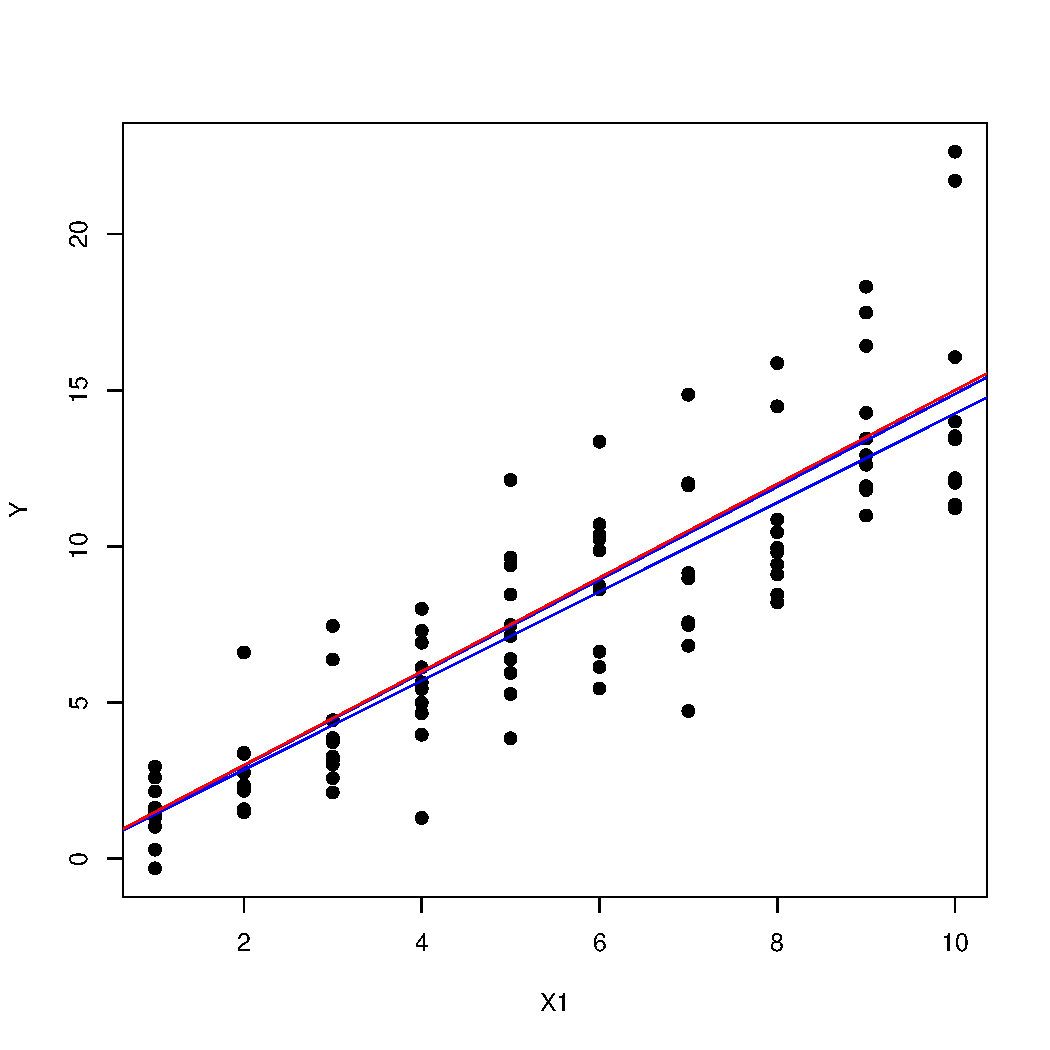
\includegraphics[width=\maxwidth]{figure/unnamed-chunk-8} 

\end{knitrout}

\end{frame}

\begin{frame}[fragile]{Heteroskedasticity is controlled through the alpha parameter}
\begin{knitrout}
\definecolor{shadecolor}{rgb}{0.969, 0.969, 0.969}\color{fgcolor}\begin{kframe}
\begin{alltt}
PaidAM0 = \hlfunctioncall{newTriangleModel}(Friedland, Response = \hlstring{"IncrementalPaid"}, 
    Predictor = \hlstring{"EP"}, FitCategory = \hlstring{"DevInteger"}, 
    Tail = 6, Alpha = 1)
PaidAM0 = \hlfunctioncall{newTriangleModel}(Friedland, Response = \hlstring{"IncrementalPaid"}, 
    Predictor = \hlstring{"EP"}, FitCategory = \hlstring{"DevInteger"}, 
    Tail = 6, Alpha = 2)
\end{alltt}
\end{kframe}
\end{knitrout}

\end{frame}

\begin{frame}[fragile]{Diagnostics pitfalls}
Following is an example, created by Francis Anscombe, of the difficulty in interpreting diagnostics




\end{frame}

\begin{frame}[fragile]{Anscombe pt.2}
\begin{knitrout}
\definecolor{shadecolor}{rgb}{0.969, 0.969, 0.969}\color{fgcolor}\begin{kframe}
\begin{alltt}
fit1 = \hlfunctioncall{lm}(y1 ~ x1)
fit2 = \hlfunctioncall{lm}(y2 ~ x2)
fit3 = \hlfunctioncall{lm}(y3 ~ x3)
fit4 = \hlfunctioncall{lm}(y4 ~ x4)
\end{alltt}
\end{kframe}
\end{knitrout}

\end{frame}

\begin{frame}[fragile]
\begin{knitrout}
\definecolor{shadecolor}{rgb}{0.969, 0.969, 0.969}\color{fgcolor}\begin{kframe}
\begin{alltt}
\hlfunctioncall{summary}(fit1)$r.squared
\end{alltt}
\begin{verbatim}
## [1] 0.6665
\end{verbatim}
\begin{alltt}
\hlfunctioncall{summary}(fit2)$r.squared
\end{alltt}
\begin{verbatim}
## [1] 0.6662
\end{verbatim}
\begin{alltt}
\hlfunctioncall{summary}(fit3)$r.squared
\end{alltt}
\begin{verbatim}
## [1] 0.6663
\end{verbatim}
\begin{alltt}
\hlfunctioncall{summary}(fit4)$r.squared
\end{alltt}
\begin{verbatim}
## [1] 0.6667
\end{verbatim}
\end{kframe}
\end{knitrout}

\end{frame}

\begin{frame}[fragile]
\begin{knitrout}
\definecolor{shadecolor}{rgb}{0.969, 0.969, 0.969}\color{fgcolor}\begin{kframe}
\begin{alltt}
op = \hlfunctioncall{par}(mfrow = \hlfunctioncall{c}(2, 2))
\hlfunctioncall{plot}(y1 ~ x1, pch = 19)
\hlfunctioncall{abline}(fit1$coefficients[[1]], fit1$coefficients[[2]])

\hlfunctioncall{plot}(y2 ~ x2, pch = 19)
\hlfunctioncall{abline}(fit1$coefficients[[1]], fit1$coefficients[[2]])

\hlfunctioncall{plot}(y3 ~ x3, pch = 19)
\hlfunctioncall{abline}(fit1$coefficients[[1]], fit1$coefficients[[2]])

\hlfunctioncall{plot}(y4 ~ x4, pch = 19)
\hlfunctioncall{abline}(fit1$coefficients[[1]], fit1$coefficients[[2]])

\hlfunctioncall{par}(op)
\end{alltt}
\end{kframe}
\end{knitrout}

\end{frame}

\begin{frame}[fragile]
\begin{knitrout}
\definecolor{shadecolor}{rgb}{0.969, 0.969, 0.969}\color{fgcolor}
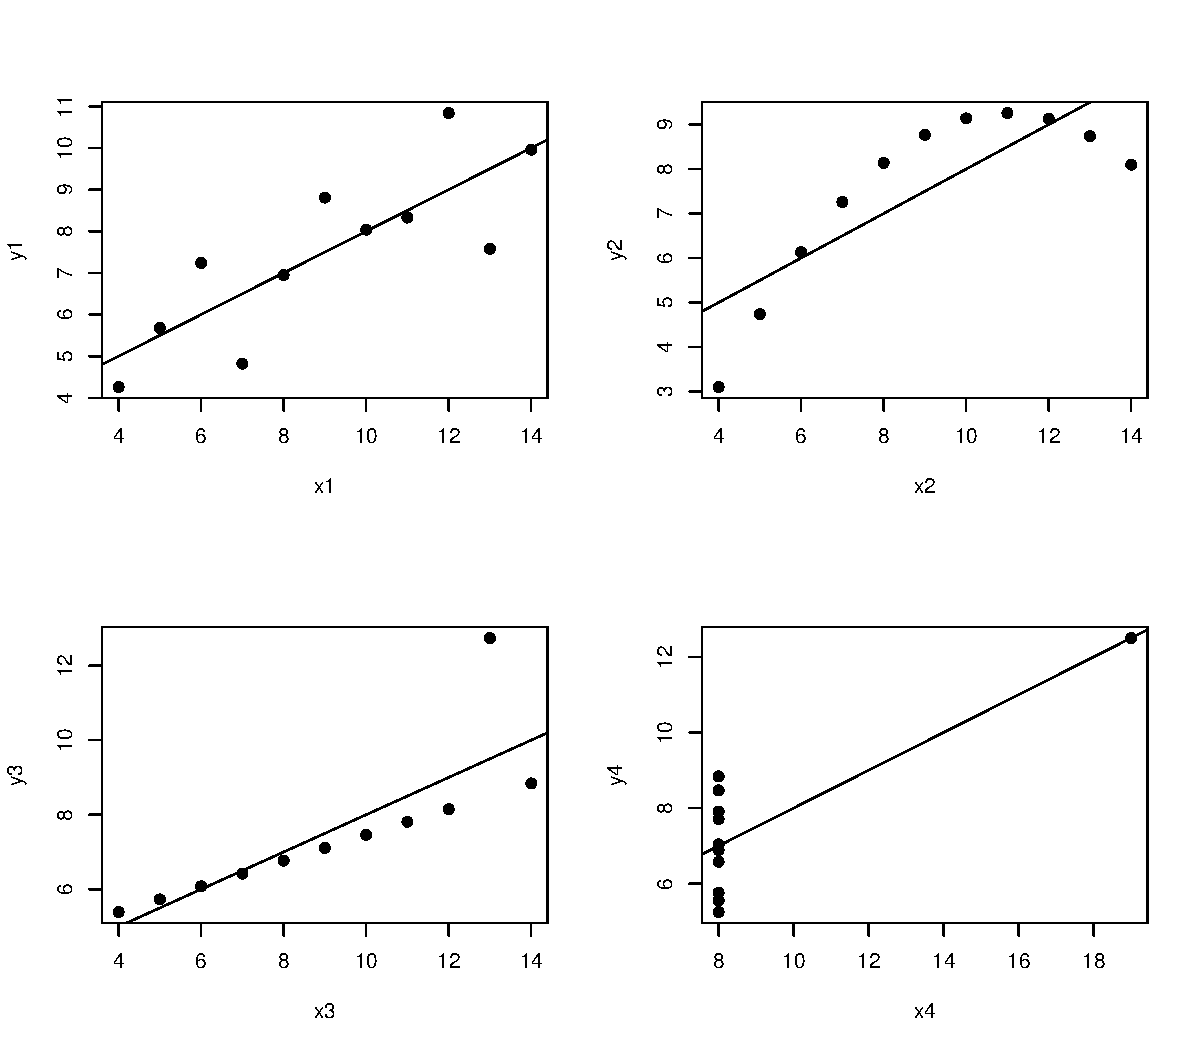
\includegraphics[width=\maxwidth]{figure/Anscombe4} 

\end{knitrout}

\end{frame}

\begin{frame}[fragile]{Observe the residual plots}
\begin{knitrout}
\definecolor{shadecolor}{rgb}{0.969, 0.969, 0.969}\color{fgcolor}\begin{kframe}
\begin{alltt}
\hlfunctioncall{PlotResiduals}(PaidAM)
\end{alltt}
\end{kframe}
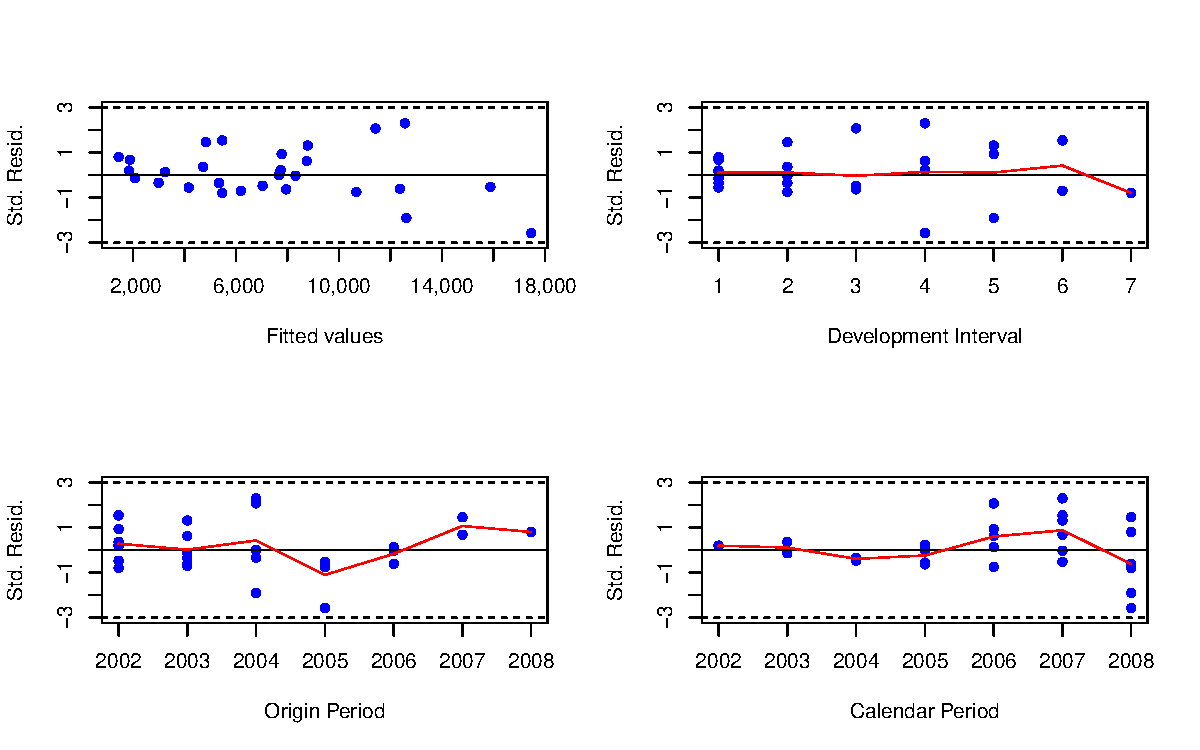
\includegraphics[width=\maxwidth]{figure/ResidualPlotsAM2} 

\end{knitrout}

\end{frame}

\begin{frame}[fragile]{Observe the residual plots}
\begin{knitrout}
\definecolor{shadecolor}{rgb}{0.969, 0.969, 0.969}\color{fgcolor}\begin{kframe}
\begin{alltt}
\hlfunctioncall{PlotResiduals}(PaidCL)
\end{alltt}
\end{kframe}
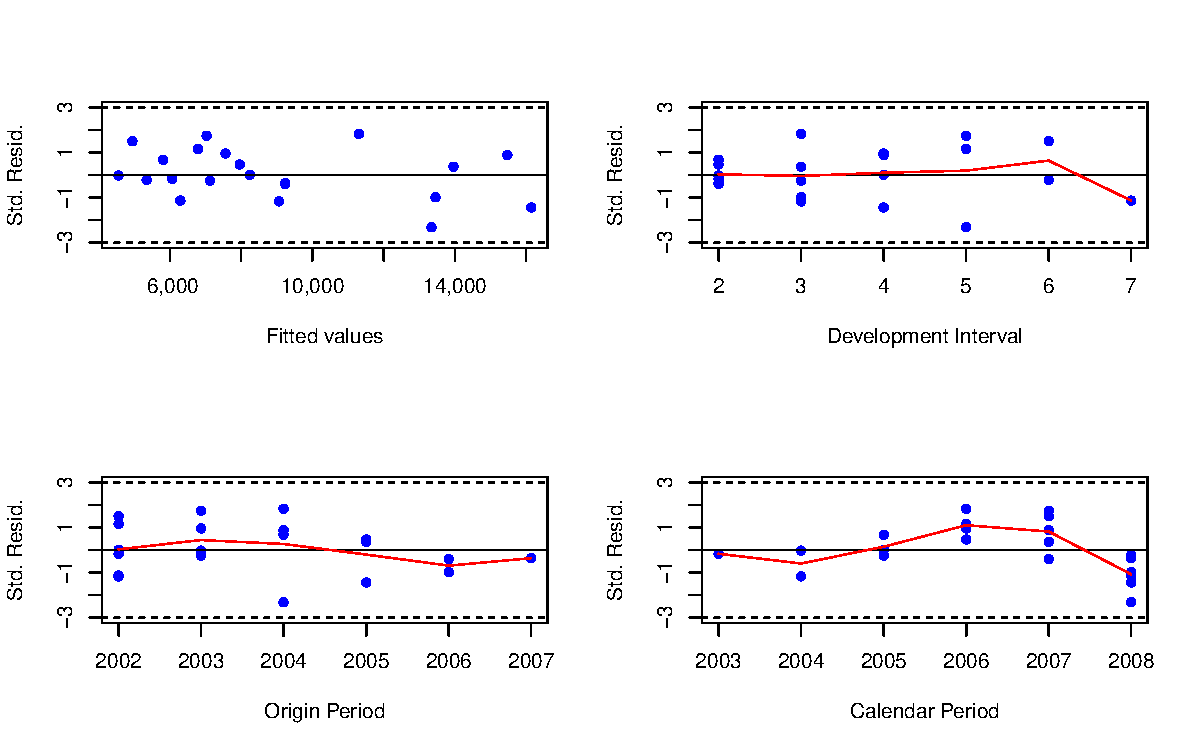
\includegraphics[width=\maxwidth]{figure/ResidualPlotsCL} 

\end{knitrout}

\end{frame}

\begin{frame}[fragile]{Projection to as-of date}
Once a model has been checked and selected, projection of losses is trivial. MRMR will either project to a specific date or a specific development lag.
\begin{knitrout}
\definecolor{shadecolor}{rgb}{0.969, 0.969, 0.969}\color{fgcolor}\begin{kframe}
\begin{alltt}
PaidAM_Projection = \hlfunctioncall{TriangleProjection}(PaidAM, 
    ProjectToDev = FALSE, AsOfDate = \hlfunctioncall{mdy}(\hlstring{"12/31/2010"}))
\end{alltt}


{\ttfamily\noindent\itshape\color{messagecolor}{\#\# estimate only: convert to intervals for accuracy}}\begin{alltt}
df = PaidAM_Projection@ProjectionData
\end{alltt}
\end{kframe}
\end{knitrout}

\end{frame}

\begin{frame}[fragile]{Projection to development age}
\begin{knitrout}
\definecolor{shadecolor}{rgb}{0.969, 0.969, 0.969}\color{fgcolor}\begin{kframe}
\begin{alltt}
PaidAM_Projection = \hlfunctioncall{TriangleProjection}(PaidAM, 
    ProjectToDev = TRUE, MaxDev = 10)
\end{alltt}


{\ttfamily\noindent\itshape\color{messagecolor}{\#\# estimate only: convert to intervals for accuracy}}\begin{alltt}
df = PaidAM_Projection@ProjectionData
\end{alltt}
\end{kframe}
\end{knitrout}

\end{frame}

\begin{frame}[fragile]{Another view of linear regression}
The ordinarly least squares (OLS) regression procedure began by minimizing the sum of squared errors. Assuming homoskedastic normal error terms, this produces the same model factors as maximizing the likelihood function.
\newline
\newline
This idea allows us to extend the model so that functional forms other than homoskedastic normal may be contemplated. Generalized linear models are one such example.
\end{frame}

\begin{frame}[fragile]{Another view of linear regression}
\begin{knitrout}
\definecolor{shadecolor}{rgb}{0.969, 0.969, 0.969}\color{fgcolor}\begin{kframe}
\begin{alltt}
\hlfunctioncall{set.seed}(1234)
N = 100
e = \hlfunctioncall{rnorm}(N, mean = 0, sd = 1)

lnLike = \hlfunctioncall{function}(x, mu, sigma) \{
    n = \hlfunctioncall{length}(x)
    lnLike = -n/2 * \hlfunctioncall{log}(2 * pi)
    lnLike = lnLike - n/2 * \hlfunctioncall{log}(sigma^2)
    lnLike = lnLike - 1/(2 * sigma^2) * \hlfunctioncall{sum}((x - 
        mu)^2)
    lnLike
\}
\end{alltt}
\end{kframe}
\end{knitrout}

\end{frame}

\begin{frame}[fragile]
\begin{knitrout}
\definecolor{shadecolor}{rgb}{0.969, 0.969, 0.969}\color{fgcolor}\begin{kframe}
\begin{alltt}
testMu = \hlfunctioncall{seq}(-0.5, 0.5, length.out = 100)
likelihood = \hlfunctioncall{sapply}(testMu, lnLike, x = e, 
    sigma = 1)
testMu[likelihood == \hlfunctioncall{max}(likelihood)]
\end{alltt}
\begin{verbatim}
## [1] -0.1566
\end{verbatim}
\end{kframe}
\end{knitrout}

\end{frame}

\begin{frame}[fragile]
\begin{knitrout}
\definecolor{shadecolor}{rgb}{0.969, 0.969, 0.969}\color{fgcolor}\begin{kframe}
\begin{alltt}
\hlfunctioncall{plot}(likelihood ~ testMu, pch = 19)
\hlfunctioncall{abline}(v = 0)
\hlfunctioncall{abline}(v = testMu[likelihood == \hlfunctioncall{max}(likelihood)])
\end{alltt}
\end{kframe}
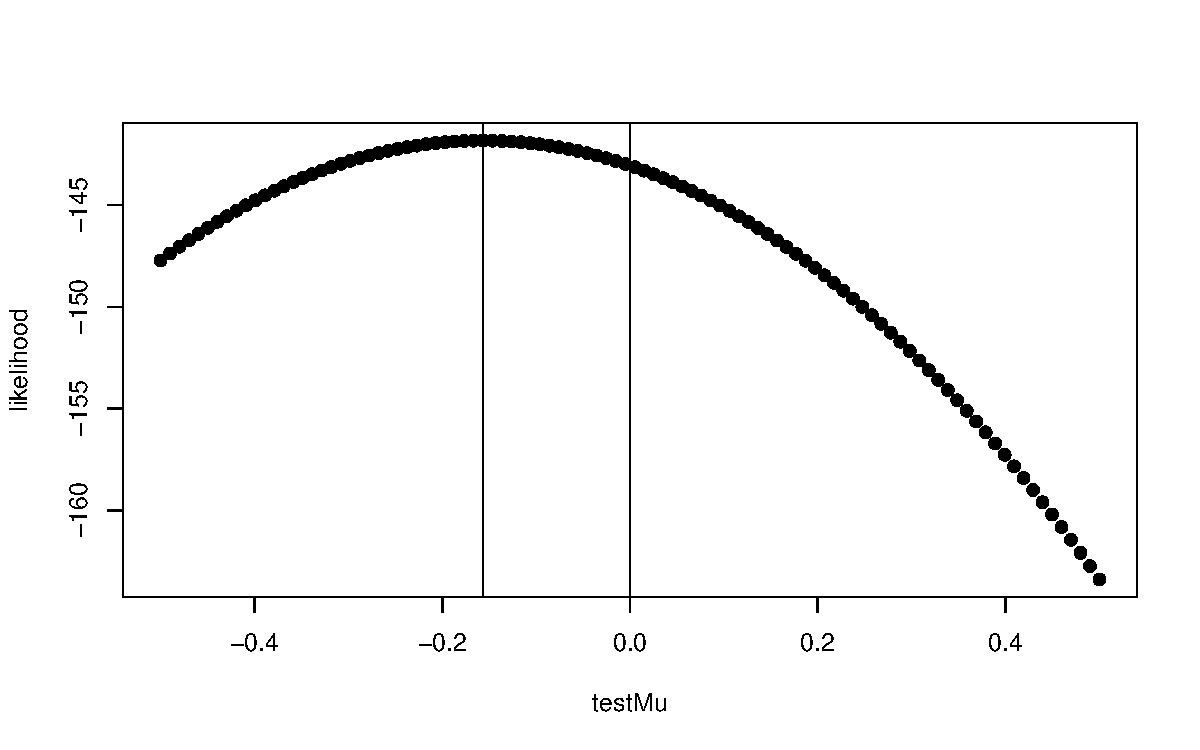
\includegraphics[width=\maxwidth]{figure/unnamed-chunk-11} 

\end{knitrout}

\end{frame}

\begin{frame}[fragile]
\begin{knitrout}
\definecolor{shadecolor}{rgb}{0.969, 0.969, 0.969}\color{fgcolor}\begin{kframe}
\begin{alltt}
testSigma = \hlfunctioncall{seq}(0.5, 1.5, length.out = 100)
likelihood = \hlfunctioncall{sapply}(testSigma, lnLike, x = e, 
    mu = 0)
testSigma[likelihood == \hlfunctioncall{max}(likelihood)]
\end{alltt}
\begin{verbatim}
## [1] 1.015
\end{verbatim}
\end{kframe}
\end{knitrout}

\end{frame}

\begin{frame}[fragile]
\begin{knitrout}
\definecolor{shadecolor}{rgb}{0.969, 0.969, 0.969}\color{fgcolor}\begin{kframe}
\begin{alltt}
\hlfunctioncall{plot}(likelihood ~ testSigma, pch = 19)
\hlfunctioncall{abline}(v = 1)
\hlfunctioncall{abline}(v = testSigma[likelihood == \hlfunctioncall{max}(likelihood)])
\end{alltt}
\end{kframe}
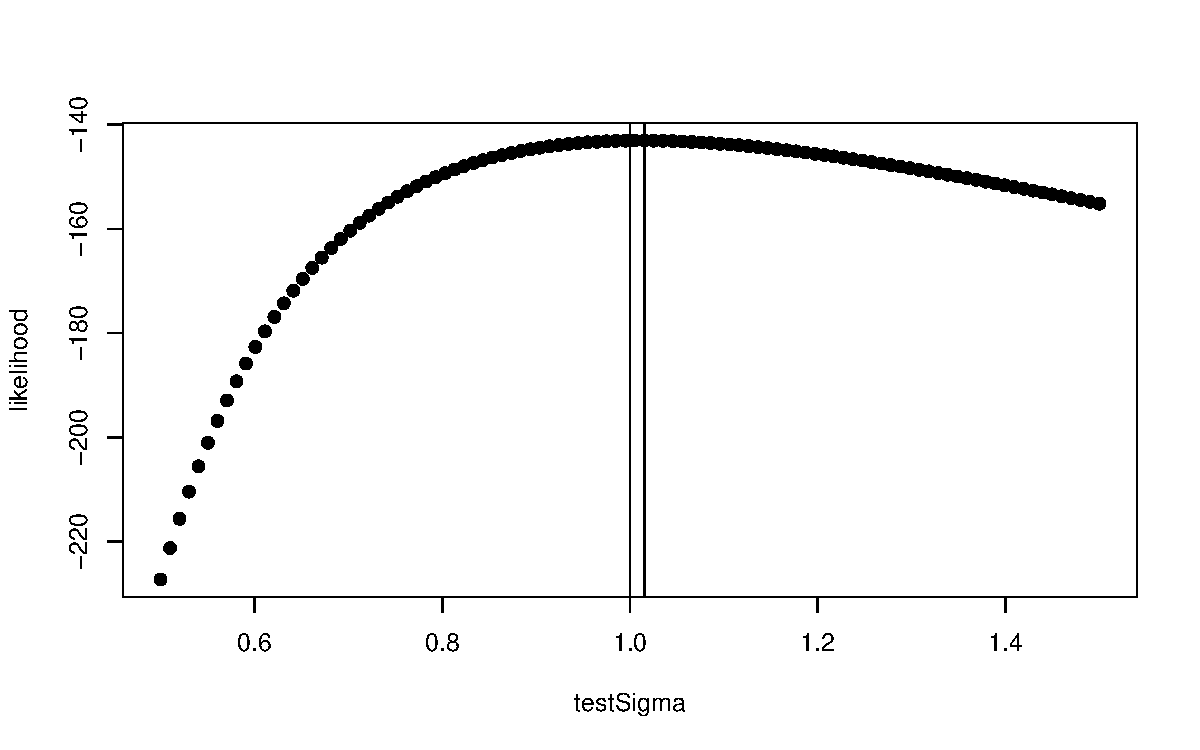
\includegraphics[width=\maxwidth]{figure/PlotSigma} 

\end{knitrout}

\end{frame}

\begin{frame}[fragile]
\begin{knitrout}
\definecolor{shadecolor}{rgb}{0.969, 0.969, 0.969}\color{fgcolor}\begin{kframe}
\begin{alltt}
params = \hlfunctioncall{expand.grid}(mu = testMu, sigma = testSigma)
params$Likelihood = \hlfunctioncall{mapply}(lnLike, params$mu, 
    params$sigma, MoreArgs = \hlfunctioncall{list}(x = e))
z = \hlfunctioncall{matrix}(params$Likelihood, \hlfunctioncall{length}(testMu), 
    \hlfunctioncall{length}(testSigma))
\end{alltt}
\end{kframe}
\end{knitrout}

\end{frame}

\begin{frame}[fragile]
\begin{knitrout}
\definecolor{shadecolor}{rgb}{0.969, 0.969, 0.969}\color{fgcolor}\begin{kframe}
\begin{alltt}
\hlfunctioncall{filled.contour}(x = testMu, y = testSigma, 
    z = z, color.palette = heat.colors, xlab = \hlstring{"mu"}, 
    ylab = \hlstring{"sigma"})
\end{alltt}
\end{kframe}
\end{knitrout}

\end{frame}

\begin{frame}[fragile]
\begin{knitrout}
\definecolor{shadecolor}{rgb}{0.969, 0.969, 0.969}\color{fgcolor}
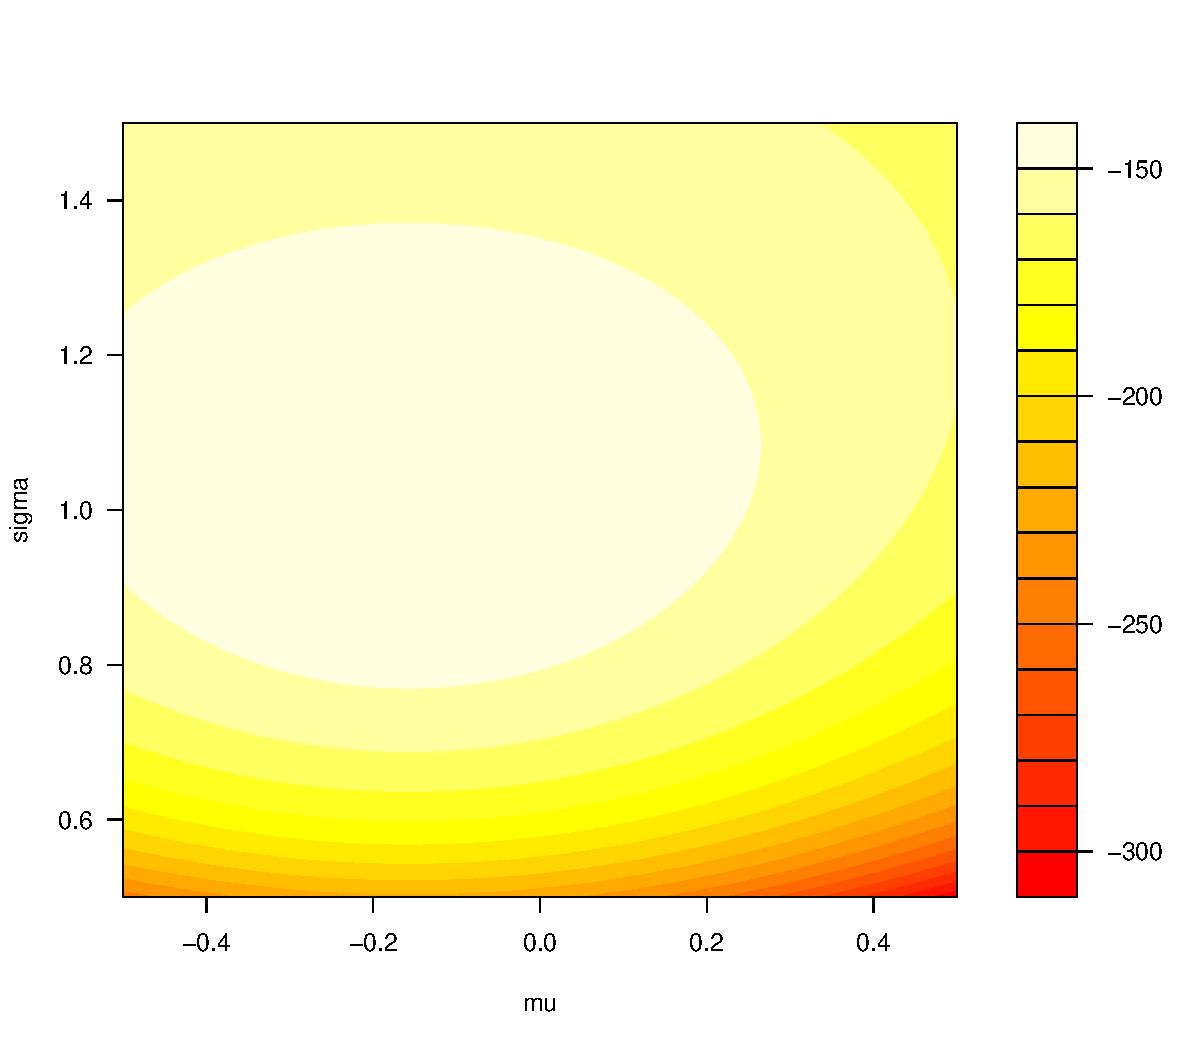
\includegraphics[width=\maxwidth]{figure/TwoDimPlotOutput} 

\end{knitrout}

\end{frame}

\begin{frame}[fragile]{Optimize for both parameters}
\begin{knitrout}
\definecolor{shadecolor}{rgb}{0.969, 0.969, 0.969}\color{fgcolor}\begin{kframe}
\begin{alltt}
lnLike2 = \hlfunctioncall{function}(x, par) \{
    mu = par[1]
    sigma = par[2]
    
    \hlfunctioncall{lnLike}(x, mu, sigma)
\}

optimFit = \hlfunctioncall{optim}(par = \hlfunctioncall{c}(-1, 4), fn = lnLike2, 
    control = \hlfunctioncall{list}(fnscale = -1), x = e)
optimFit$par
\end{alltt}
\begin{verbatim}
## [1] -0.1566  0.9994
\end{verbatim}
\end{kframe}
\end{knitrout}

\end{frame}

\begin{frame}[fragile]{Add a constant term to the normal variable e}
\begin{knitrout}
\definecolor{shadecolor}{rgb}{0.969, 0.969, 0.969}\color{fgcolor}\begin{kframe}
\begin{alltt}
B0 = 5
Y = B0 + e
\end{alltt}
\end{kframe}
\end{knitrout}

\end{frame}
 
\begin{frame}[fragile]{This is equivalent to lm}
\begin{knitrout}
\definecolor{shadecolor}{rgb}{0.969, 0.969, 0.969}\color{fgcolor}\begin{kframe}
\begin{alltt}
optimFit = \hlfunctioncall{optim}(par = \hlfunctioncall{c}(-1, 4), fn = lnLike2, 
    control = \hlfunctioncall{list}(fnscale = -1), x = Y)
optimFit$par[[1]]
\end{alltt}
\begin{verbatim}
## [1] 4.843
\end{verbatim}
\begin{alltt}

lmFit = \hlfunctioncall{lm}(Y ~ 1)
lmFit$coefficients[[1]]
\end{alltt}
\begin{verbatim}
## [1] 4.843
\end{verbatim}
\end{kframe}
\end{knitrout}

\end{frame}

\begin{frame}[fragile]{Now add a slope}
\begin{knitrout}
\definecolor{shadecolor}{rgb}{0.969, 0.969, 0.969}\color{fgcolor}\begin{kframe}
\begin{alltt}
X = \hlfunctioncall{as.double}(1:\hlfunctioncall{length}(e))
B1 = 1.5
Y = B0 + B1 * X + e

lnLike3 = \hlfunctioncall{function}(par, Y, X) \{
    B0 = par[1]
    B1 = par[2]
    sigma = par[3]
    
    x = Y - B0 - B1 * X
    mu = 0
    
    \hlfunctioncall{lnLike}(x, mu, sigma)
\}
\end{alltt}
\end{kframe}
\end{knitrout}

\end{frame}

\begin{frame}[fragile]
\begin{knitrout}
\definecolor{shadecolor}{rgb}{0.969, 0.969, 0.969}\color{fgcolor}\begin{kframe}
\begin{alltt}
optimFit = \hlfunctioncall{optim}(par = \hlfunctioncall{c}(4, 1, 1), fn = lnLike3, 
    control = \hlfunctioncall{list}(fnscale = -1), Y = Y, 
    X = X)
optimFit$par[1:2]
\end{alltt}
\begin{verbatim}
## [1] 4.404 1.509
\end{verbatim}
\begin{alltt}

lmFit = \hlfunctioncall{lm}(Y ~ 1 + X)
lmFit$coefficients
\end{alltt}
\begin{verbatim}
## (Intercept)           X 
##       4.406       1.509
\end{verbatim}
\end{kframe}
\end{knitrout}

\end{frame}

\begin{frame}{Further}
  \begin{itemize}
    \item Coursera
    \item Meetup.com
    \item R-bloggers.com
      \begin{itemize}
        \item PirateGrunt.com
        \item MagesBlog.com
      \end{itemize}
    \item Github
    \item Books!
    \begin{itemize}
      \item Machine Learning for Hackers by Conway \& White
      \item Software for Data Analysis by Chambers
      \item Data Analysis Using Regression and Multilevel/Hierarchical Models by Gelman \& Hille
      \item Introduction to the Theory and Practice of Econometrics by Judge, Griffiths \& Hill
    \end{itemize}
    \item Other languages
    \begin{itemize}
      \item Python
      \item D3
    \end{itemize}
  \end{itemize}
\end{frame}

\end{document}
